\zag{Введение}

\subzag{Предмет и метод молекулярной оптики}
\vskip 2mm

Молекулярная оптика есть часть физики, посвященная изучению
процессов взаимодействия электромагнитного излучения с веществом,
процессов, определяемых микроскопической структурой вещества и
молекулярной динамикой газов, жидкостей, растворов,
кристаллов и жидких кристаллов.

Эта самостоятельная область знаний характеризуется единым методом
исследования большого многообразия явлений, которые удалось
истолковать в рамках электронной теории, учитывающей строение,
электрические и оптические свойства атомов и молекул. Задача этой
области науки заключается в том, чтобы выразить свойства среды
через молекулярные константы. Обратная задача исходит из
утверждения возможности установить однозначную связь между
свойствами молекул и свойствами среды. Это возможно, если
молекулы сохраняют в среде свою индивидуальность (слабое
межмолекулярное взаимодействие). Молекулярная оптика изучает
следующий ряд явлений, связанных с важнейшей характеристикой
молекулы --- ее поляризуемостью: преломление, отражение и
поглощение света изотропными и анизотропными средами;
дисперсия света; рассеяние света; естественная оптическая
активность молекул; вынужденное двойное лучепреломление в силовых
полях: в электрическом --- явление Керра, в магнитном --- явление
Коттон-Мутона, в поле градиента скорости --- явление Максвелла. В
молекулярной оптике устанавливается связь между этими явлениями.
Все они в той или иной мере определяются тензором 2-ого ранга ---
поляризуемостью молекулы.

В настоящее время мы имеем возможность вводимые в молекулярную
оптику феноменологические константы (составляющие тензора
поляризуемости) выразить через величины, непосредственно
характеризующие строение электронной оболочки молекулы. Такими
величинами являются характеристики энергетических уровней и
вероятности перехода между ними.

В конечном счете, ключ к раскрытию сущности оптических свойств
молекулы дают частоты и интенсивности в ее спектре. поэтому в
основе молекулярной оптики лежит молекулярная спектроскопия.
Физические величины, характеризующие свойства микроскопических
объектов --- атомов и молекул, --- могут быть определены
теоретически только при помощи квантовой механики.
Квантовомеханическая теория явлений молекулярной оптики, в
частности явления дисперсии света, хорошо разработана и приводит
к таким же результатам, что и классическая теория. Это позволяет
пользоваться классической полуэмпирической теорией
молекулярно-оптических явлений, дающей не только качественное, но
и количественное их объяснение, и вскрывающей их внутренние
связи. Эта теория основывается, с одной стороны, на общих
положениях электромагнитной теории света и свойствах
излучающего электрона, с другой --- на химической теории строения
молекул.

Таким образом, молекулярно-оптическими называются такие явления,
в которых находят свое отражение не только свойства света, но и
свойства среды, с которой он взаимодействует. Тем самым, явления
молекулярной оптики представляют один из наиболее важных
источников информации о строении и свойствах молекул, жидкостей,
кристаллов, высокомолекулярных веществ и коллоидных систем. Этим
определяется большое прикладное значение молекулярной оптики, ее
применение в технике, в различных областях физики, химии,
метеорологии, астрономии.

\subzag{Основные законы электромагнитной теории света}%@@@
\vskip 2mm Далее предполагается, что читатель уже знаком с
основами теории электромагнитного поля. Поэтому приводятся лишь
основные положения электромагнитной теории света.

Электромагнитная волна в вакууме характеризуется значениями
векторов напряженности электрического поля $\vec E$ и магнитного
поля $\vec H$. В веществе электромагнитное поле световой волны
характеризуется векторами электрической и магнитной индукции $\vec
D$ и $\vec B$, векторами $\vec E$ и $\vec H$, плотностью
электрических зарядов $\rho$, а также (в случае проводников)
плотностью тока проводимости $\vec j$. Свойства электромагнитного
поля передаются уравнениями Максвелла:
\begin{plain}$$\eqalign{\rot\vec H=&{1\over c}{\partial\vec D\over\partial t}
+{4\pi\over c}\vec j,\cr \rot\vec E=&-{1\over c}{\partial\vec
B\over\partial t},\cr \diverg\vec D=&4\pi\rho,\cr \diverg\vec
B=&0.}\noq$$\end{plain} Здесь $c$ --- скорость света в вакууме
($3\cdot10^{10}\ {\rm см\cdot сек^{-1}}$). Связь между пятью
векторами поля дается соотношениями (справедливыми для изотропной
среды):
\begin{plain}$$\eqalign{\vec j=&\sigma\vec E,\cr
\vec D=&\varepsilon\vec E,\cr \vec B=&\mu\vec H.}\noq$$\end{plain} Здесь
$\sigma$ --- электропроводность, $\varepsilon$ --- диэлектрическая
постоянная и $\mu$ --- магнитная проницаемость вещества. Величины
$\varepsilon$ и $\mu$ безразмерны, электропроводность имеет
размерность ${\rm сек^{-1}}$. В общем случае анизотропного тела
электропроводность, диэлектрическая постоянная и магнитная
восприимчивость анизотропны и выражаются тензорами. Рассматриваем,
главным образом, взаимодействие со светом немагнитных
диэлектриков, для которых $\sigma=0$ и $\mu=0$. Связь между
индукцией и напряженностью может быть выражена и иначе,
посредством вектора поляризации вещества (электрической или
магнитной). Имеем в электрическом поле:
$$\vec D=\varepsilon\vec E=\vec E+4\pi\vec P,\noq$$
или
$$\vec P={\varepsilon-1\over4\pi}\vec E.\noq$$
Вектор $\vec P$ характеризует электрический дипольный момент
единицы объема вещества. Объемная плотность энергии
электромагнитного поля равна:
$$W={1\over8\pi}\vec E\vec D+{1\over8\pi}\vec H\vec B.\noq$$
Напряженности поля могут быть выражены через потенциалы поля.
Введу вихревого характера магнитного поля, можно положить:
$$\vec B=\rot\vec A,\noq$$
где $\vec A$ --- вектор-потенциал поля. Подставляя это уравнение
во второе уравнение \eqn{1}, получаем:
$$\rot\left(\vec E+{1\over c}{\partial\vec A\over\partial
t}\right)=0.\noq$$ Уравнение \eqn{7} удовлетворяется выражением:
$$\vec E=-{1\over c}{\partial\vec A\over\partial
t}-\grad\varphi.\noq$$ Так как ротор от градиента скаляра
тождественно равен нулю: $\rot\,\grad\varphi\equiv0$, то $\varphi$
--- скалярный потенциал поля.
\par\noindent Уравнение \eqn{6} определяет ротор вектор-потенциала. Задав
дивергенцию в виде
$$\diverg\vec A=-{\varepsilon\mu\over c}{\partial\varphi\over\partial
t},\noq$$ получаем из уравнений Максвелла уравнения для
потенциалов:
\begin{plain}$$\eqalign{\nabla^2\vec A-{\varepsilon\mu\over
c^2}{\partial^2\vec A\over\partial t^2}=&-{4\pi\mu\over c}\vec
j,\cr \nabla^2\varphi-{\varepsilon\mu\over
c^2}{\partial^2\varphi\over\partial t^2}=&-{4\pi\over\varepsilon}
\rho.}\noq$$\end{plain} В отсутствие свободных зарядов и токов оба потенциала
удовлетворяют волновому уравнению:
$$c'={c\over\sqrt{\varepsilon\mu}},\hskip 5mm\nabla^2\Psi={1\over
{c'}^2}{\partial^2\Psi\over\partial t^2}.\noq$$
Сферически-симметричное решение волнового уравнения описывает
сферическую электромагнитную волну:
$$\Psi={1\over R}\left\{f_1\left(t-{R\over c'}\right)+f_2
\left(t+{R\over c'}\right)\right\},\noq$$ где $f_1,\ f_2$ ---
произвольные функции. Первый член \eqn{12} представляет
сферическую волну, исходящую из некоторого источника поля и
распространяющуюся со скоростью $c'$; второй --- волну, приходящую
из бесконечности и сходящуюся в истоке поля. Нас будет
интересовать только первая часть решения \eqn{12}:
$$\Psi={1\over R}f\left(t-{R\over c'}\right).\eqno (1.12a)$$
Источниками переменного электромагнитного поля служат движущиеся
заряды. Решение \eqn{12{\it a}} в явной форме имеет вид:
\begin{plain}$$\eqalign{\varphi=&{1\over R}\int{\rho\left(t-{R\over
c'}\right)\over R}dV\cr \vec A=&{\mu\over c}\int{\vec
j\left(t-{R\over c'}\right)\over R}dV}.\noq$$\end{plain} Интегрирование
проводится по всему объему. Для нахождения поля в некоторой точке
в момент $t$ нужно для каждого элемента объема $dV$ определить тот
заряд и ток, которые находились в $dV$ в момент $\left(t-{R\over
c'}\right)$ где $R$ --- расстояние от $dV$ до точки, в которой
определяется поле.

Потенциалы \eqn{13} --- запаздывающие потенциалы. Сферическая
волна уносит из излучающего объема определенное количество
энергии. Если потеря энергии происходит только посредством
излучения, то мы можем написать:
$$-{\partial W\over\partial t}={\partial\over\partial
t}\int{\omega dV}=-{1\over8\pi}{\partial\over\partial t}\int(\vec
E\vec D+\vec H\vec B)dV=\int\limits_{S}S_ndS,\noq$$ где $S_n$ ---
проекция вектора потока энергии на нормаль к элементу поверхности
$dS$, охватывающий излучающий объем. Вектор потока энергии
называется вектором Умова-Пойнтинга:
$$\vec S={c\over4\pi}[\vec E\vec H].\noq$$
Для того, чтобы получить непосредственные выражения $\vec E$ и
$\vec H$ сферической электромагнитной волны, необходимо, очевидно,
задаться определенной характеристикой излучателя. Однако, так или
иначе, ясно, что на достаточно большом удалении от излучателя
ограниченный участок сферической волны может считаться плоским.
Следовательно, если $z$ есть направление нормали к этому участку
--- направление распространения волны, имеем:
$$\vec E=\vec E(z,t);\hskip 4mm\vec H=\vec H(z,t),\noq$$
и, считая волну монохроматической, т.е. зависящей от времени по
гармоническому закону, получаем:
$$\vec E=\vec E(z)e^{iwt};\hskip 4mm \vec H=\vec
H(z)e^{iwt}.\eqno (1.16a)$$ Рассмотрим плоскую волну в однородном
диэлектрике, лишенном свободных зарядов. Из \eqn{1} и \eqn{2}
имеем:
$${\varepsilon\over c}{\partial\vec E\over\partial t}=\rot\vec
H.$$ Дифференцируя это уравнение по времени и подставляя в него
значение ${\partial\vec H\over\partial t}$ из второго уравнения
\eqn{1}, получаем в конце концов:
$${\varepsilon\mu\over c^2}{\partial^2\vec E\over\partial
t^2}=\nabla^2\vec E,\noq$$ и аналогично:
$${\varepsilon\mu\over c^2}{\partial^2\vec Н\over\partial
t^2}=\nabla^2\vec H.\eqno (1.17a)$$ Подставляя \eqn{16{\it a}} в
\eqn{17} и \eqn{17{\it a}}, находим:
\begin{plain}$$\eqalign{\vec E=&\vec E_{01}e^{i(wt-kz)}+\vec
E_{02}e^{i(wt+kz)},\cr \vec H=&\vec H_{01}e^{i(wt-kz)}+\vec
H_{02}e^{i(wt+kz)}}.\noq$$\end{plain} Здесь $k=w{\sqrt{\varepsilon\mu}\over
c}={w\over c'}={2\pi\nu\over c'}={2\pi\over
c'T}={2\pi\over\lambda}$, $T$
--- период, $\lambda$ --- длина волны в среде, связанная с длиной
волны в вакууме $\lambda_0$ соотношением:
$$\lambda={c'\over c}\lambda_0.\noq$$
Первые члены \eqn{18} описывают плоскую электромагнитную волну,
распространяющуюся вдоль положительного, вторые --- волну,
распространяющуюся вдоль отрицательного направления $z$.
Ограничимся рассмотрением первых членов. В общем случае можем
написать:
$$\vec E=\vec E_0e^{iw(t-{\vec r\vec s\over c'})}=\vec
E_0e^{i(wt-\vec k\vec r)},\noq$$ и аналогично для $\vec H$. Здесь
$\vec s$ --- единичный вектор нормали к волне, $\vec k$ ---
волновой вектор:
$$\vec k={2\pi\vec s\over \lambda}.$$
Подставляя \eqn{20} в уравнения Максвелла, после несложных
преобразований находим:
$$\vec E\vec s=0,\hskip 4mm\vec H\vec s=0, \hskip 4mm\vec E\vec
H=0.\noq$$ Эти уравнения выражают поперечность световой волны и
взаимную перпендикулярность $\vec E$ и $\vec H$.

Световая волна может характеризоваться различными состояниями
поляризации. У естественного света плоскости, в которых колеблются
перпендикулярные друг другу векторы $\vec E$ и $\vec H$, не
фиксированы, и между составляющими этих векторов нет определенных
соотношений вследствие хаотического разброса поляризаций отдельных
волновых цугов. В усреднении по времени:
$$\overline{E_x^2}=\overline{E_y^2}=\overline{E_z^2},\hskip 4mm
\overline{E_xE_y}=\overline{E_yE_z}=\overline{E_zE_x}=0,$$ и
аналогично для $H$.

Плоско(линейно)-поляризованная волна характеризуется определенным
направлением колебаний векторов $\vec E$ и $\vec H$. При этом
плоскостью поляризации световой волны принято называть плоскость,
в которой колеблется магнитный вектор, иными словами, плоскость,
перпендикулярную к плоскости колебаний электрического вектора.
Если отдельные составляющие волны \eqn{20}характеризуются
различными значениями фазы, волна в общем случае, является
эллиптически поляризованной.

Пусть $s=s_z$ и (в вещественной форме)
\begin{plain}$$\eqalign{E_x=&A_1\cos(\tau+\delta_1)\cr
E_y=&A_2\cos(\tau+\delta_2)}$$\end{plain} Здесь $\tau=w\left(t-{\vec r\vec
s\over c'}\right)$. Исключая $\tau$ находим:
$$\left({E_x\over A_1}\right)^2+\left({E_y\over
A_2}\right)^2-2{E_x\over A_1}{E_y\over
A_2}\cos(\delta_2-\delta_1)=\sin^2(\delta_2-\delta_1).\noq$$ Это
уравнение является уравнением эллипса. В частном случае, при
$\delta_2-\delta_1=2n{\pi\over2}$ имеем линейную поляризацию, а в
случае $A_1=A_2$ и $\delta_2-\delta_1=(2n+1){\pi\over2}$ ---
круговую ($n=0,\pm1,\pm2,...$). Если
$\delta_2-\delta_1={\pi\over2}+2|n|\pi$, т.е.
\begin{plain}$$\eqalign{E_x=&A\cos(\tau+\delta_1),\cr
E_y=&-A\sin(\tau+\delta_1),}$$\end{plain} волна --- правая, а если
$\delta_2-\delta_1=-{\pi\over2}+2|n|\pi$, т.е.
\begin{plain}$$\eqalign{E_x=&A\cos(\tau+\delta_1),\cr
E_y=&A\sin(\tau+\delta_1),}$$\end{plain} волна --- левая. Если смотреть
навстречу распространяющейся волне, то в первой волне
электрический вектор обходит окружность по направлению часовой
стрелки. В комплексной форме эллиптически поляризованная волна
характеризуется соотношением вида
$${E_y\over E_x}=a+bi,$$
причем, для линейно поляризованной волны $b=0$. В случае правой и
левой круговой волны соответственно:
$${E_y\over E_x}=i,\hskip 4mm{E_y\over E_x}=-i.$$
Нетрудно установить соотношение между $a$ и $b$, с одной стороны,
и $A_1,\ A_2$ и $(\delta_2-\delta_1)$ --- с другой.

К этому мы вернемся далее.

\subzag{Тензор поляризуемости.} \vskip 2mm Оптические свойства
среды (немагнитного диэлектрика) характеризуются в общем
анизотропном случае тензором диэлектрической постоянной для
электромагнитных волн. В изотропной среде согласно
электромагнитной теории света, диэлектрическая постоянная связана
с показателем преломления соотношением:
$$\varepsilon=n^2.$$
Согласно \eqn{3},
$$\varepsilon\vec E=\vec E+4\pi\vec P.$$
Вектор поляризации $\vec P$ выражает дипольный момент единицы
объема среды, в которой имеется поле $\vec E$. Если $N_1$ ---
число молекул в единице объема, то
$$\vec P=N_1\vec p_{\varepsilon},$$
где $\vec p_{\varepsilon}$ --- дипольный момент молекулы в
направлении поля. В быстропеременном электрическом поле световой
волны $\vec p_{\varepsilon}$ возникает лишь вследствие индукции
зарядов, но не благодаря ориентации полем дипольных молекул, так
как при больших частотах изменения поля молекулы не успевают
ориентироваться (дисперсия).

Индуцированный электрическим полем дипольных момент пропорционален
напряженности поля:
$$\vec p_{\varepsilon}=\alpha\vec E,\noq$$
$$\vec P=N_1\alpha\vec E.\eqno (1.23a)$$
Коэффициент $\alpha$ выражает индукционную, электронную
поляризуемость молекулы --- способность ее электронов смещаться
под действием поля $\vec E$. Из соотношения \eqn{23} следует
написать соотношения:
$$p_i=\sum\limits_{k}\alpha_{ik}E_k,\hskip 4mm i,k=x,y,z.\noq$$
Коэффициенты $\alpha_{ik}$ являются, тем самым, составляющими
тензора второго ранга. Тензор $\alpha_{ik}$ может быть
комплексным, что означает, очевидно, несовпадение фазы дипольного
момента $p_i$ с фазой действующей напряженности поля $E_k$. Такое
несовпадение может определяться, в частности, наличием вызванного
теми или иными причинами затухания колебаний электронов. В этом
случае в молекуле действуют неконсервативные силы и некоторая
часть энергии электромагнитного поля поглощается --- имеет место
поглощение света. Исследуя вещество в спектральной области,
достаточно удаленной от собственных полос поглощения, можем
отвлечься от действия этих сил. В отсутствии поглощения света
рассматриваемая система является консервативной, и тензор
поляризуемости $\alpha_{ik}$ должен быть эрмитовым, т.е. должно
соблюдаться условие:
$$\alpha_{ik}=\alpha_{ki}^*.\noq$$
Следовательно, диагональные составляющие тензора $\alpha_{ii}$
обязательно вещественны.

Докажем, что консервативной системе должен соответствовать эрмитов
тензор поляризуемости.

Общее выражение для энергии поляризующейся молекулы в
электрическом поле имеет вид:
$$U={1\over2}\vec p\vec
E^*={1\over2}\sum\limits_{i,k}\alpha_{ik}E_i^*E_k.\noq$$ Это
выражение вещественно, каким и должно быть выражение для энергии.
Коэффициент ${1\over2}$ возникает при интегрировании:
$$U(x)=\int\limits_{0}^{E_x}p_xdE_x=\int\limits_{0}^{E_x}
\sum\limits_{k}\alpha_{xk} E_xdE_x={1\over2}p_xE_x.$$ Очевидно,
что
$$U^*=U={1\over2}\sum\limits_{i,k}\alpha_{ik}^*E_iE_k^*={1\over2}\sum
\limits_{i,k}\alpha_{ik}E_i^*E_k.$$ И, так как сумма не меняется
от перестановки индексов $i,k$:
$$U={1\over2}\sum\limits_{i,k}\alpha_{ik}E^*_iE_k={1\over2}\sum_{i,k}\alpha^*_{ik}
E^*_iE_k.$$ Условия \eqn{25} достаточно, чтобы удовлетворить этому
соотношению. Докажем, что оно необходимо.

Пусть на молекулу действует сила поля $E_x^*$, возрастающая от 0
до $E_x^*$. Работа, производимая этой силой, есть вещественная
величина, равная
$$A_{1x}=\int\limits_{0}^{E_x^*}p_xdE_x^*=\int\limits_{0}^{E_x^*}\alpha_{xx}E_xdE_x^*=
{1\over2}\alpha_{xx}|E_x|^2.$$ Подействуем теперь силой $E_y^*$,
возрастающей от 0 до $E_y^*$. Получим работу:
$$A_{1y}=\int\limits_{0}^{E_{y}^*}p_ydE_y^*=\int\limits_{0}^{E_y^*}(\alpha_{yx}
E_x+\alpha_{yy}E_y)dE_y^*=\alpha_{yx}E_xE_y^*+{1\over2}a_{yy}|E_y|^2.$$
Общая работа равна:
$$A_1=A_{1x}+A_{1y}={1\over2}\alpha_{xx}|E_x|^2+\alpha_{yx}E_xE_y^*+{1\over2}
\alpha_{yy}|E_y|^2.$$ Проведем теперь тот же процесс в обратном
порядке:
$$A_{2y}=\int\limits_{0}^{E_y^*}p_ydE_y^*=\int\limits_0^{E_y^*}\alpha_{yy}E_ydE^*_y=
{1\over2}\alpha_{yy}|E_y|^2,$$
$$A_{2x}=\int\limits_0^{E_x^*}p_xdE_x^*=\int\limits_0^{E_x^*}(\alpha_{xy}E_y+
\alpha_{xx}E_x)dE_x^*=\alpha_{xy}E_yE_x^*+{1\over2}\alpha_{xx}|E_x|^2,$$
$$A_2=A_{2y}+A_{2x}={1\over2}\alpha_{yy}|E_y|^2+\alpha_{xy}E_x^*E_y+{1\over2}\alpha_{xx}|E_x|^2.$$
Для консервативной системы вещественные величины $A_1=A_2$, и,
следовательно, $\alpha_{yx}=\alpha_{xy}^*$. Аналогичным образом
находим
$$\alpha_{zx}=\alpha_{xz}^*,\hskip 4mm\alpha_{zy}=\alpha_{yz}^*,$$
что и требовалось доказать.

Вещественная часть тензора поляризуемости, в силу его эрмитовости,
есть его симметричная часть:
$$S_{ik}={1\over2}\left(\matrix{
\alpha_{xx}&\alpha_{xy}&\alpha_{xz}\cr
\alpha_{yx}&\alpha_{yy}&\alpha_{yz}\cr
\alpha_{zx}&\alpha_{zy}&\alpha_{zz}\cr
}\right)+{1\over2}\left(\matrix{
\alpha_{xx}&\alpha_{xy}^*&\alpha_{xz}^*\cr
\alpha_{yx}^*&\alpha_{yy}&\alpha_{yz}^*\cr
\alpha_{zx}^*&\alpha_{zy}^*&\alpha_{zz}\cr }\right)=\left(\matrix{
\alpha_{xx}&{\alpha_{xy}+\alpha_{xy}^*\over2}&\alpha_{xz}^*\cr
{\alpha_{yx}+\alpha_{yx}^*\over2}&\alpha_{yy}&{\alpha_{yz}+\alpha_{yz}^*\over2}\cr
{\alpha_{zx}+\alpha_{zx}^*\over2}&{\alpha_{zy}+\alpha_{zy}^*\over2}&\alpha_{zz}\cr
}\right).$$ Действительно, согласно \eqn{25} этот тензор
симметричен и равен:
$$\left(\matrix{
\alpha_{xx}&\alpha'_{xy}&\alpha'_{xz}\cr
\alpha'_{yx}&\alpha_{yy}&\alpha'_{yz}\cr
\alpha'_{zx}&\alpha'_{zy}&\alpha_{zz}\cr }\right),\noq$$ где
$$\alpha'_{xy}={1\over2}(\alpha_{xy}+\alpha_{xy}^*)=
{1\over2}(\alpha_{yx}+\alpha_{yx}^*)={1\over2}(\alpha_{xy}+\alpha_{yx})$$
--- вещественные величины.

Напротив, мнимая часть эрмитова тензора ассиметрична:
$$A_{ik}={1\over2}\left(\matrix{
\alpha_{xx}&\alpha_{xy}&\alpha_{xz}\cr
\alpha_{yx}&\alpha_{yy}&\alpha_{yz}\cr
\alpha_{zx}&\alpha_{zy}&\alpha_{zz}\cr
}\right)-{1\over2}\left(\matrix{
\alpha_{xx}&\alpha_{xy}^*&\alpha_{xz}^*\cr
\alpha_{yx}^*&\alpha_{yy}&\alpha_{yz}^*\cr
\alpha_{zx}^*&\alpha_{zy}^*&\alpha_{zz}\cr
}\right)=$$$$=\left(\matrix{
0&{\alpha_{xy}-\alpha_{xy}^*\over2}&{\alpha_{xz}-\alpha_{xz}^*\over2}\cr
{\alpha_{yx}-\alpha_{yx}^*\over2}&0&{\alpha_{yz}-\alpha_{yz}^*\over2}\cr
{\alpha_{zx}-\alpha_{zx}^*\over2}&{\alpha_{zy}-\alpha_{zy}^*\over2}&0\cr
}\right)=\left(\matrix{ 0&\alpha''_{xy}&\alpha''_{xz}\cr
-\alpha''_{yx}&0&\alpha''_{yz}\cr
-\alpha''_{zx}&-\alpha''_{zy}&0\cr }\right).\noq$$ Здесь
$\alpha''_{xy}={1\over2}(\alpha_{xy}-\alpha_{xy}^*)={1\over
2}(\alpha_{xy}-\alpha_{yx})=-\alpha''_{yx}$ --- чисто мнимые
величины. Составляющие тензора второго ранга при преобразовании
координат преобразуются, как произведение двух векторов. Очевидно,
что выражение $\alpha_{xy}-\alpha_{yx}$ преобразуется как $z$-овая
составляющая векторного произведения или аксиального вектора
$${1\over2}(\alpha_{xy}-\alpha_{yx})=i[\vec b\vec c]_z=id_z,$$
и ассиметричная часть эрмитова тензора приводится к виду
$$A_{ik}=i\left(\matrix{
0&d_z&-d_y\cr -d_z&0&d_x\cr d_y&-d_x&0\cr }\right).\eqno (1.28a)$$
Следовательно, $\alpha_{ik}=S_{ik}+A_{ik}$, или
\begin{plain}$$\eqalign{\alpha_{xy}=&S_{xy}+i[\vec b\vec c]_z=S_{xy}+id_z,\cr
\alpha_{yx}=&S_{xy}-i[\vec b\vec c]_z=S_{xy}-id_z},$$\end{plain} и т.д.

Во всех задачах молекулярной оптики, за исключением относящихся к
магнитному и естественному вращению плоскости поляризации света,
мы будем, в отсутствии поглощения света, иметь дело с вещественным
и, следовательно, симметричным тензором $S_{ik}$, для которого
сохраним обозначение $\alpha_{ik}$. Такому тензору соответствует
вещественный эллипсоид поляризуемости
$$\sum\limits_{x',y'}\alpha'_{x'y'}x'y'={\rm const}.\noq$$
Соответствующим поворотом осей координат этот эллипсоид может быть
преобразован к главным осям:
$$\sum\limits_x \alpha_{xx}x^2={\rm const}.\noq$$
Иными словами, тензор преобразуется к диагональной форме:
$$S_{ik}=i\left(\matrix{
\alpha_{xx}&0&0\cr 0&\alpha_{yy}&0\cr 0&0&\alpha_{zz}\cr
}\right).\eqno (1.27a)$$ Напомним, каким образом осуществляется
это преобразование. Нужно найти направления главных осей
координат, в которых тензор принимает форму \eqn{27{\it a}}.
Следовательно, задача сводится к нахождению трех взаимно
ортогональных векторов, которые при умножении на тензор
\eqn{27{\it a}} не меняли бы своего направления, а изменялись бы
только по величине. При умножении на $S_{ik}$ произвольного
вектора, очевидно, получается новый вектор, вообще говоря, другой
величины и направления.

Итак, ищем вектор $\vec A$, удовлетворяющий условию:
$$(S_{ik})\vec A=\Lambda\vec A,\noq$$
или
$$\sum\limits_k\alpha'_{ik}A_{ik}=\Lambda A_i.\eqno (1.31a)$$
Таких уравнений три:
\begin{plain}$$\eqalign{\alpha'_{xx}A_x+\alpha'_{xy}A_y+\alpha'_{xz}A_z=&\Lambda
A_x,\cr \alpha'_{xy}A_x+\alpha'_{yy}A_y+\alpha'_{yz}A_z=&\Lambda
A_y,\cr \alpha'_{xz}A_x+\alpha'_{yz}A_y+\alpha'_{zz}A_z=&\Lambda
A_z.}$$\end{plain} Условием разрешимости системы однородных уравнений
является равенство определителя системы нулю. Имеем вековое
уравнение:
$$\left|\matrix{
\alpha'_{xx}-\Lambda&\alpha'_{xy}&\alpha'_{xz}\cr
\alpha'_{xy}&\alpha'_{yy}-\Lambda&\alpha'_{yz}\cr
\alpha'_{xz}&\alpha'_{yz}&\alpha'_{zz}-\Lambda }\right|.\noq$$
Коэффициенты $\Lambda$ являются корнями векового уравнения
\eqn{32}. Легко показать, что три вектора $\vec A$,
соответствующие трем корням  $\Lambda_1,\Lambda_2,\Lambda_3$,
взаимно ортогональны. Эти три вектора $\vec A_1,\vec A_2,\vec A_3$
таковы, что любой вектор, совпадающий по направлению с $\vec A_1,$
$\vec A_2$ или $\vec A_3$, при умножении на $S_{ik}$ не
поворачивается, а только изменяет свое численное значение. если мы
повернем оси координат так, чтобы они совпадали с $A_1,A_2,A_3$,
получим тензор:
$$\left(\matrix{
\Lambda_1&0&0\cr 0&\Lambda_2&0\cr 0&0&\Lambda_3 }\right),\noq$$
тождественный тензору \eqn{27a}. Иными словами:
$$\alpha_{xx}=\Lambda_1,\hskip 4mm\alpha_{yy}=\Lambda_2,\hskip
4mm\alpha_{zz}=\Lambda_3.$$ Таким образом, математическая задача
приведения вещественного тензора к главным осям сводится к решению
векового уравнения \eqn{32}:
$$\Lambda^3-(\alpha'_{xx}+\alpha'_{yy}+\alpha'_{zz})\Lambda^2
-\left\{\left|\matrix{ \alpha'_{xx}&\alpha'_{xy}\cr
\alpha'_{xy}&\alpha'_{yy} }\right|+\left|\matrix{
\alpha'_{yy}&\alpha'_{yz}\cr \alpha'_{yz}&\alpha'_{zz}
}\right|+\left|\matrix{ \alpha'_{zz}&\alpha'_{xz}\cr
\alpha'_{xz}&\alpha'_{xx} }\right|\right\}\Lambda+$$ $$+\left|\matrix{
\alpha'_{xx}&\alpha'_{xy}&\alpha'_{xz}\cr
\alpha'_{xy}&\alpha'_{yy}&\alpha'_{yz}\cr
\alpha'_{xz}&\alpha'_{yz}&\alpha'_{zz}}\right|=0.\noq$$
Инвариантами преобразования \eqn{27}$\rightarrow$\eqn{33} в силу
свойств кубического уравнения являются следующие выражения:

-- след тензора --- сумма его диагональных членов:
$$b=\alpha'_{xx}+\alpha'_{yy}+\alpha'_{zz}=\Lambda_1+\Lambda_2+\Lambda_3
\equiv\alpha_{xx}+\alpha_{yy}+\alpha_{zz};\noq$$

-- сумма трех миноров, соответствующих диагональным членам:
$$B=\left|\matrix{
\alpha'_{xx}&\alpha'_{xy}\cr \alpha'_{xy}&\alpha'_{yy}
}\right|+\left|\matrix{ \alpha'_{yy}&\alpha'_{yz}\cr
\alpha'_{yz}&\alpha'_{zz} }\right|+\left|\matrix{
\alpha'_{zz}&\alpha'_{xz}\cr \alpha'_{xz}&\alpha'_{xx}
}\right|=\Lambda_1\Lambda_2+\Lambda_2\Lambda_3+\Lambda_3\Lambda_1;\noq$$

-- определитель тензора:
$$D=\left|\matrix{
\alpha'_{xx}&\alpha'_{xy}&\alpha'_{xz}\cr
\alpha'_{xy}&\alpha'_{yy}&\alpha'_{yz}\cr
\alpha'_{xz}&\alpha'_{yz}&\alpha'_{zz}}\right|=\Lambda_1\Lambda_2\Lambda_3.\noq$$
Очевидно, что любая комбинация $b$, $B$ и $D$ также будет
инвариантом. Важными инвариантами являются:
$$A=b^2-2B=\Lambda^2_1+\Lambda_2^2+\Lambda_3^2\equiv\alpha_{xx}^2+\alpha_{yy}^2
+\alpha_{zz}^2=$$ $$=\alpha'^2_{xx}+\alpha'^2_{yy}+\alpha'^2_{zz}+2(\alpha'^2_{xy}+
\alpha'^2_{yz}+\alpha'^2_{xz}),$$ и
$$g^2=A-B=b^2-3B=$$ $$={1\over2}\left\{(\alpha_{xx}-\alpha_{yy})^2
+(\alpha_{yy}-\alpha_{zz})^2+(\alpha_{zz}-\alpha_{xx})^2\right\}={3\over
2}\sum\limits_{i,k}\alpha'^2_{ik}-{1\over 2}\left(\sum\limits_i
\alpha'_{ii}\right)^2.\noq$$ Инвариант $g$ носит название
анизотропии тензора. В частном случае изотропно поляризующейся
системы эллипсоид поляризуемости обращается в шар и
$\Lambda_1=\Lambda_2=\Lambda_3=0$; $g=0$. Тензор поляризуемости
вырождается в скаляр. Возможен случай $\Lambda_1;\
\Lambda_2=\Lambda_3$. При этом эллипсоид поляризуемости есть
эллипсоид вращения. В общем случае имеем дело с трехосным
эллипсоидом.

Легко видеть, что вещественный асимметричный тензор имеет мнимые
главные оси, так как корни векового уравнения
$$\left|\matrix{
-\Lambda&\alpha'_{xy}&\alpha'_{xz}\cr
\alpha'_{xy}&-\Lambda&\alpha'_{yz}\cr
\alpha'_{xz}&\alpha'_{yz}&-\Lambda}\right|=0$$ мнимые.

\subzag{Свойства среды и свойства молекул.} \vskip 2mm Обычная
постановка проблемы в молекулярной оптике, как и в других областях
молекулярной физики, такова: выразить свойства среды через
молекулярные постоянные, т.е. через свойства молекул, из которых
состоит вещество. Обратная, не менее важная задача заключается в
определении молекулярных постоянных, свойств молекул из свойств
среды в целом.

Реальный макроскопический объем вещества в наших экспериментах
содержит весьма большое число молекул. Исходное положение
молекулярной теории, положение, без которого сама молекулярная
физика не могла бы существовать, состоит в признании возможности
установить однозначную связь между свойствами среды и свойствами
молекул. Это положение справедливо в непосредственной форме лишь
до тех пор, пока молекулы сохраняют в среде свои индивидуальные
свойства, т.е. пока силы межмолекулярного взаимодействия
значительно слабее внутримолекулярных сил, определяемых строением
электронных оболочек молекул. Однако статистический метод Гиббса в
принципе позволяет решить задачу и при сколь угодно большом
межмолекулярном взаимодействии. Ясно, какое большое значение имеет
для молекулярной физики изучение межмолекулярного взаимодействия,
всегда имеющего место в реальном веществе. Зная природу
межмолекулярного взаимодействия , умея связывать ее со свойствами
молекул, мы получаем возможность решить основную задачу
молекулярной физики и в тех случаях, когда межмолекулярное
взаимодействие велико --- в случае жидкостей и кристаллов.

В общем случае связь между свойствами вещественной среды и
свойствами молекул носит статистический характер. Благодаря этому
возникают физические понятия, имеющие смысл только применительно к
среде в целом, но не к отдельным молекулам. Таким понятием
является, например, температура, которая на основе
газокинетической теории может быть выражена через среднюю
кинетическую энергию молекул. Оптические постоянные среды
(например, показатель преломления) оказываются связанными с
усредненными значениями молекулярных постоянных (поляризуемости).
В частном случае усреднение может сводиться к простому
суммированию --- так, внутренняя энергия тела есть сумма энергий
молекул. Наконец, возможны случаи, в которых свойства среды в
целом совпадают со свойствами отдельных частиц. Не имеет смысла
говорить о температуре молекулы, но можно говорить об ее спектре:
так, например, спектр газа в целом, грубо говоря, совпадает со
спектром каждой из молекул. Это не более как частный случай общей
статистической  связи. Если вещество находится при достаточно
высокой температуре, его спектр представится наложением спектров
молекул, статистически распределенных по различным энергетическим
уровням. Контур спектральной линии в значительной мере
определяется свойствами среды. В задачах молекулярной оптики мы
встречаемся, главным образом, с необходимостью статистического
усреднения по различным ориентациям молекул в пространстве. Если
речь идет о свободном газе, то усреднение проводится по всем
ориентациям, являющимся равновероятными. В жидкости существует
ближний порядок в расположении молекул, поэтому задача усреднения
существенно усложняется.

В случае изотропного вещества, находящегося под действием внешнего
поля, это действие необходимо учитывать при усреднении. В
кристалле частицы ориентированы определенным образом и эта
определенная ориентация должна учитываться явно и непосредственно.

Величинами, подлежащими усреднению по различным пространственным
ориентациям молекул, в оптике являются, прежде всего, составляющие
тензора поляризуемости молекулы $\alpha_{ik}$. Задача сводится к
усреднению положений системы координат, закрепленной в молекуле
--- молекулярно-неподвижной (в качестве таковой рационально
выбрать систему главных осей эллипсоида поляризуемости),
относительно системы координат, закрепленной в пространстве и
задаваемой самой постановкой опыта пространственно-неподвижной
системы (одна из осей которой --- направление распространения
световой волны)(рис. 1.1). Взаимное расположение молекулярной и
пространственной систем координат выражается направляющими
косинусами одной системы в другой.\vskip -2mm

\vskip 3mm
\centerline{\hbox{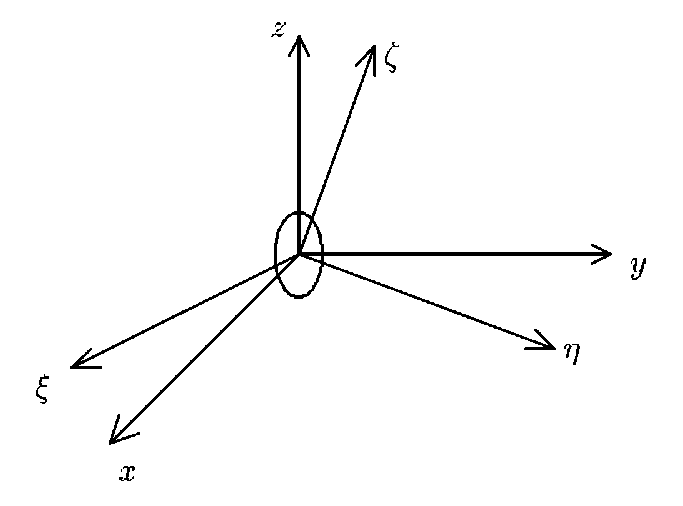
\includegraphics[scale=0.7]{Ris/ris_eps/ris1_01.eps}}}

\centerline{\ris Рис. 1.1. Молекулярная и
пространственная системы координат.} \vskip 1mm

В дальнейшем будем обозначать координаты пространственной системы
буквами $x,y,z$ (индексы $i,k$ и т.д.), координаты молекулярной
системы --- буквами $\xi,\eta,\zeta$ (индексы $\sigma,\tau$ и
т.д.) или цифрами 1,2,3. Удобнее всего выражать направляющие
косинусы $(\sigma i)$ через углы Эйлера $\varphi,\psi,\vartheta$
(рис. 1.2).\vskip -2mm

\vskip 3mm
\centerline{\hbox{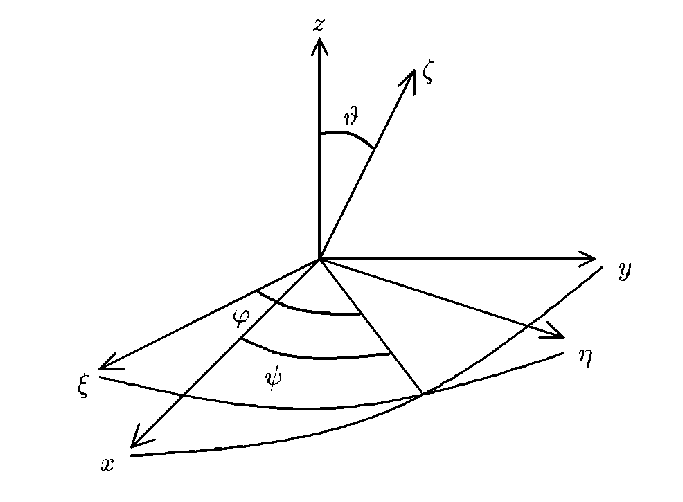
\includegraphics[scale=0.7]{Ris/ris_eps/ris1_02.eps}}}

\centerline{\ris Рис 1.2. Углы Эйлера.} \vskip 2mm
Имеем таблицу значений направляющих косинусов (табл. 1.1). \vskip
1mm {\ris Таблица 1.1.} 
\vskip 3mm
\centerline{\hbox{\includegraphics[scale=1]{Ris/ris_eps/tab1_01.eps}}}

\leftskip 0cm Во всех задачах мы столкнемся с необходимостью
усреднения различных выражений, содержащих направляющие косинусы,
по всевозможным расположениям системы $\sigma$ относительно
системы $i$. Считая эти расположения равновесными, имеем:
$$f\left\{(\sigma i),(\tau k),\hbox{...}\right\}=
{\int\limits_{0}^{2\pi}\int\limits_{0}^{2\pi}\int\limits_{0}^{\pi}
fd\varphi d\psi \sin\vartheta d\vartheta\over
\int\limits_{0}^{2\pi}\int\limits_{0}^{2\pi}\int\limits_{0}^{\pi}
d\varphi d\psi \sin\vartheta d\vartheta}={1\over 8\pi^2}
\int\limits_{0}^{2\pi}\int\limits_{0}^{2\pi}\int\limits_{0}^{\pi}
fd\varphi d\psi \sin\vartheta d\vartheta.\noq$$ Нам придется иметь
дело с функциями $f$ от направляющих косинусов в первой, второй,
третьей и четвертой степени. Легко видеть, что
$$\overline{(\sigma i)}=\overline{(\zeta
z)}=\overline{\cos\vartheta}=0,\noq$$ так же сразу находим
$$\overline{(\sigma i)^2}=\overline{(\zeta
z)^2}=\overline{\cos^2\vartheta}={1\over3},$$ и
$$\overline{(\sigma i)(\sigma j)}=\overline{(\sigma i)(\tau
j)}=\overline{(\sigma i)(\tau i)}=0,$$ или
$$\overline{(\sigma i)(\tau
j)}={1\over3}\delta_{\sigma\tau}\delta_{ij}. \noq$$ Из функций
третьего порядка отличны от нуля только произведения направляющих
косинусов, не содержащие повторяющихся индексов:
$$\overline{(\xi x)(\eta y)(\zeta z)}=
\overline{(\eta x)(\zeta y)(\xi z)}=\overline{(\zeta x)(\xi
y)(\eta z)}=$$$$= -\overline{(\xi x)(\eta y)(\zeta
z)}=-\overline{(\eta x)(\xi y)(\zeta z)}= -\overline{(\zeta
x)(\eta y)(\xi z)}={1\over6}.\noq$$ Функции четвертого порядка,
отличные от нуля:
\begin{plain}$$\eqalign{
&\overline{(\sigma i)^4}={1\over5},\cr &\overline{(\sigma
i)^2(\tau i)^2}=\overline{(\sigma i)^2(\sigma j)^2}={1\over15},\cr
&\overline{(\sigma i)^2(\tau j)^2}={2\over15},\cr
&\overline{(\sigma i)(\sigma j)(\tau i)(\tau j)}={1\over30},\cr
&\sigma\not=\tau,\hskip 4mm i\not=j }.\noq$$\end{plain} Все эти результаты
могут быть получены непосредственным интегрированием \eqn{38}, с
учетом эквивалентности всех трех осей в каждой системе координат.

\subzag{Симметрия молекул и тензор поляризуемости.} \vskip 2mm
Молекулы обладают определенной симметрией расположения атомов.
Зная симметрию молекулы, мы можем сделать ряд выводов об ее
электрических и оптических свойствах. Хотя физические свойства
молекулы определяются, в основном, строением электронных оболочек
атомов, из которых она состоит, однако, свойства симметрии в
расположении электронов и связей обязательно те же, что и в
расположении ядер.

Итак, многоатомная молекула может рассматриваться как система
точек. Точками в этом случае являются атомы, из которых она
построена. Конечная точечная система может обладать следующими
типами элементов симметрии.

Первый тип --- оси симметрии, обозначаемые $C_n$. Если при
повороте вокруг оси на угол ${2\pi\over n}$ тело совмещается само
с собой, то оно обладает осью симметрии $C_n$. В молекулах
встречаются оси следующих порядков: $n=2,3,4,5,6$ и оси полной
аксиальной симметрии $C_{\infty}$ (линейные молекулы).

Второй тип --- плоскость зеркального отражения --- тело
совмещается само с собой при отражении от некоторой плоскости.
Такая плоскость обозначается $\sigma$. Если система одновременно
обладает осью симметрии, лежащей в этой плоскости, плоскость
симметрии называется вертикальной и обозначается $\sigma_{v}$.
Если ось симметрии нормальна к плоскости $\sigma$, последняя
называется горизонтальной и обозначается $\sigma_h$.

Наконец, если самосовмещение системы достигается при повороте
вокруг некоторой оси на угол ${2\pi\over n}$ и последующим
отражении в плоскости, перпендикулярной этой оси, то система имеет
зеркально-поворотную ось $n$-ого порядка, обозначаемую $S_n$.
Порядок n в этом случае может быть только четным.
Зеркально-поворотные оси симметрии нечетного порядка являются
просто сочетанием поворотной оси того же порядка с
перпендикулярной плоскостью симметрии и не представляют собой
независимых элементов симметрии. В частном случае, если $n=2$,
самосовмещение происходит при повороте вокруг оси на угол
$180^{\circ}$, с последующим отражением в плоскости,
перпендикулярной этой оси. То же самое самосовмещение может быть
достигнуто отражением точечной системы в точке, являющейся
пересечением этой оси и плоскости --- в центре симметрии системы.
В этом случае система обладает зеркально-поворотной осью $S_2$,
или, что то же самое, центром симметрии $i$.

Таким образом, мы имеем плоскость симметрии $\sigma$, центр
симметрии $i$, обычную поворотную ось симметрии $C_n$ и
зеркально-поворотную ось $S_n$. Отнесение конкретной молекулы к
определенной группе симметрии определяется теми элементами
симметрии, которыми обладает нормальная конфигурация этой
молекулы.

\vskip 3mm
\centerline{\hbox{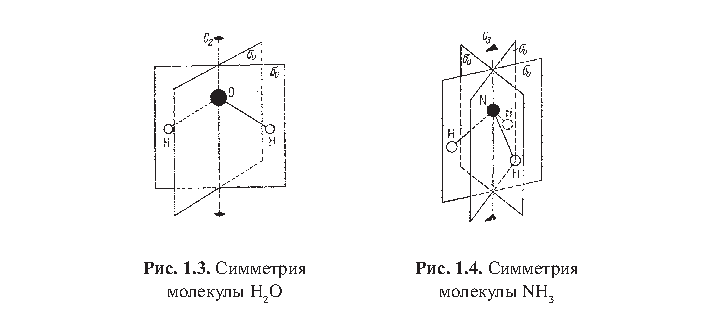
\includegraphics[scale=0.55]{Ris/ris_eps/ris1_03.eps}}}

\leftskip 0cm \centerline{\ris Рис. 1.3. Молекула группы симметрии
$C_{3v}$ ($\rm NH_3$).} \vskip 2mm Рассмотренные операции
симметрии обладают тем свойством, что они оставляют неподвижной по
крайней мере одну точку в пространстве. При отражении в центре
неподвижным является этот центр, при отражении в плоскости
неподвижными являются все точки этой плоскости, при повороте
вокруг оси неподвижными являются все точки этой оси. При сочетании
элементов симметрии одна очка обязательно остается неподвижной.
Она не обязательно совпадает в случае нормальной конфигурации
молекулы с одним из атомов. Примером может служить молекула
этилена ${\rm C_2H_4}$, для которой при операциях симметрии
неподвижным остается центр симметрии, совпадающий с серединой
двойной связи ${\rm C=C}$. Поэтому группы симметрии,
представляющие совокупность поворотов и отражений, переводящих
нормальную конфигурацию саму в себя, называют точечными группами
симметрии или просто точечными группами.

Реальная точечная система может обладать не каким-либо одним, а
несколькими различными элементами симметрии. Их определенные
комбинации автоматически вводят новые элементы симметрии. Так,
например, если система имеет ось симметрии $C_n$, и вертикальную
плоскость симметрии $\sigma_v$, то, в силу вращательной симметрии,
определяемой наличием $C_n$, обязательно присутствует еще $(n-1)$
плоскостей $\sigma_v$. Таким образом, не может быть комбинации оси
$C_n$ с одной плоскостью $\sigma_v$, но лишь комбинация оси $C_n$
с $n$ плоскостями $\sigma_v$. Примером такой системы, обладающей
симметрией $C_{3v}$ (ось $C_3$ и 3 плоскости $\sigma_v$), является
пирамидальная молекула аммиака ${\rm NH_3}$ (см. рис. 1.3). Для
молекулы воды это будет симметрия $C_{2v}$.

Наличие такого рода автоматической связи между различными
элементами симметрии приводит к тому, что число возможных типов
симметрии точечных систем оказывается ограниченным. Число типов
или групп симметрии, складывающихся из конечного числа поворотов и
отражений (следовательно, без осей $C_{\infty}$), равно
четырнадцати. Это: две простых группы $C_n$ и $S_{2n}$, содержащие
лишь одну ось (простую и зеркально-поворотную), группа $C_{nh}$,
получаемая комбинацией $C_n$ и $\sigma_h$; группа $C_{nv}$, о
которой мы уже говорили; группа диэдра $D_n$ --- комбинация $C_n$
и $n$ перпендикулярных к $C_n$ осей $C_2$, в частном случае для
$D_2$ используют обозначение $V$; группа $D_{nh}$ --- комбинация
$D_n$ и $\sigma_h\perp C_n$, $D_{2h}=V_h$; группа $D_{nd}$ ---
комбинация $D_n$ с $n$ плоскостями симметрии, проходящими между
осями второго порядка; группа $T$ --- тетраэдра, представляющая
совокупность только его осей симметрии; группа $T_d$ ---
совокупность всех элементов симметрии тетраэдра; группа $O$ ---
осей симметрии октаэдра; $T_h$ --- совокупность элементов
симметрии, представляемых диагоналями куба, тремя осями $C_2$,
проходящими через центры противоположных граней, и тремя
плоскостями симметрии, параллельными граням куба; $O_h$ ---
совокупность всех элементов симметрии куба; $J$ и $J_h$ ---
группы, являющиеся соответственно совокупностью всех осей
симметрии или всех элементов симметрии икосаэдра.

Теперь рассмотрим связь тензора поляризуемости с симметрией
молекул. Любые физические свойства молекул в значительной степени
определяются их симметрией. Как указывали раньше, физические
величины, в частности поляризуемость, выражающие свойства
анизотропного тела, имеют характер тензоров. Большинство молекул
являются оптически анизотропными. Это означает, что как величина,
так и направление индуцированного дипольного момента зависит от
ориентации молекулы в электромагнитном поле.

Пусть на произвольно ориентированную молекулу действует поле
$E_x$, которое индуцирует в молекуле дипольный момент $\vec p$,
проекции которого на оси координат пропорциональны $E_x$:
$$p_x=\alpha_{xx}E_x;\hskip 4mm p_y=\alpha_{yx}E_x;\hskip 4mm
p_z=\alpha_{zx}E_x.$$ В общем случае
$$p_i=\sum\limits_k\alpha_{ik}E_k;\hskip 4mm i,k=x,y,z\ ,\noq$$
где $\alpha_{ik}$ --- симметричный тензор второго ранга.

В каждой молекуле имеются молекулярные оси поляризуемости: 1,2,3.
То есть, если поле направлено вдоль какой-нибудь оси, то
направление $\vec p$ строго параллельно направлению этого поля:
$$\vec p_1=\alpha_1\vec E;\hskip 4mm\vec p_2=\alpha_2\vec
E;\hskip 4mm\vec p_3=\alpha_3\vec E,$$ где
$\alpha_1,\alpha_2,\alpha_3$ --- главные поляризуемости молекулы.
Знание их в молекулярной системе координат позволяет найти
компоненты тензора $\alpha_{ik}$ в любой системе координат.

Напишем формулы преобразования тензора поляризуемости от главных
молекулярных осей 1,2,3 к лабораторной системе координат.
Направление вектора $E$ задано в пространственно неподвижной
системе координат $x,y,z$. Рассмотрим дипольных момент,
индуцированный полем в молекуле, выразив составляющие момента в
молекулярной системе координат 1,2,3, совпадающей с системой
главных осей эллипсоида поляризуемости молекулы (см. рис. 1.4).

\vskip 3mm
\centerline{\hbox{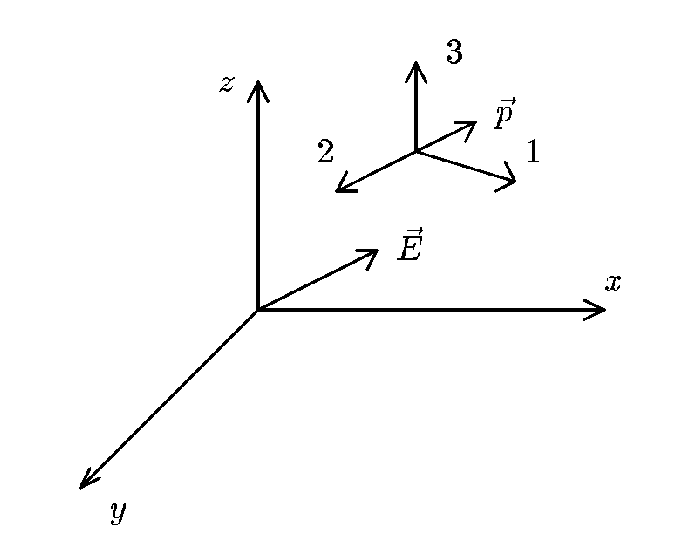
\includegraphics[scale=0.7]{Ris/ris_eps/ris1_04.eps}}}

\leftskip 0cm \centerline{\ris Рис. 1.4. Дипольный момент в
молекулярной и пространственной системах координат.} \vskip 2mm В
этой системе имеем:
$$E_{\sigma}=\sum\limits_{i=x,y,z}E_i(\sigma i),\hskip 4mm
\sigma=1,2,3\ ,\noq$$
\begin{plain}$$\eqalign{
p_{\sigma}=&\alpha_{\sigma}E_{\sigma}=\alpha_{\sigma}\sum\limits_i
E_i(\sigma i),\cr p_i=&\sum\limits_{\sigma}p_{\sigma}(\sigma i)
}.\noq$$\end{plain} Проекции вектора $\vec p$ на оси 1,2,3:
$p_1=\alpha_1E_1,\ p_2=\alpha_2E_2,\ p_3=\alpha_3E_3$, но из
формул \eqn{44-45} следует:
$$p_x=\sum\limits_{\sigma}\alpha_{\sigma}(\sigma
x)^2E_x+\sum\limits_{\sigma}\alpha_{\sigma}(\sigma x)(\sigma
y)Ey+\sum\limits_{\sigma}\alpha_{\sigma}(\sigma x)(\sigma
z)E_z.\noq$$ При сравнении выражения \eqn{46} с формулой \eqn{43},
можно сделать вывод, что они тождественно равны, если множители
при $E_x$ в формулах равны:
\begin{plain}$$\eqalign{
\alpha_{xx}=&\alpha_1(1x)^2+\alpha_{2}(2x)^2+\alpha_3(3x)^2,\cr
\alpha_{yy}=&\alpha_1(1y)^2+\alpha_{2}(2y)^2+\alpha_3(3y)^2,\cr
\alpha_{zz}=&\alpha_1(1z)^2+\alpha_{2}(2z)^2+\alpha_3(3z)^2,\cr
\alpha_{xy}=&\alpha_{yx}=\alpha_1(1x)(1y)+\alpha_{2}(2x)(2y)+\alpha_3(3x)(3y),\cr
\alpha_{xz}=&\alpha_{zx}=\alpha_1(1x)(1z)+\alpha_{2}(2x)(2z)+\alpha_3(3x)(3z),\cr
\alpha_{yz}=&\alpha_{zy}=\alpha_1(1x)(1z)+\alpha_{2}(2y)(2z)+\alpha_3(3y)(3z)
.}\noq$$\end{plain}Формулы \eqn{47} --- формулы преобразования тензора
поляризуемости от главных осей к произвольной системе координат. В
случае если одна из лабораторных осей, например ось $z$, совпадает
с осью 3, угол между этими осями равен нулю, и тогда:
$$\cos(3z)=1;\hskip 3mm\cos(3x)=\cos(3y)=\cos(1z)=\cos(2z)=0,$$
и
\begin{plain}$$\eqalign{
\alpha_{xx}=&\alpha_1(1x)^2+\alpha_2(2x)^2,\cr
\alpha_{yy}=&\alpha_1(1y)^2+\alpha_2(2y)^2;\hskip
4mm\alpha_{zz}=\alpha_2,\cr
\alpha_{xy}=&\alpha_1(1x)(1y)+\alpha_2(2x)(2y);\hskip 4mm
\alpha_{xz}=\alpha_{yz}=0. }$$\end{plain} 

Таким образом, если ось $z$
является осью тензора поляризуемости, то компоненты тензора
$\alpha_{xz}$ и $\alpha_{yz}$ равны нулю. И соответственно, если
ось $y$ --- главная ось тензора, то $\alpha_{xy}=\alpha_{zy}=0$;
если ось $x$: $\alpha_{xy}=\alpha_{xz}=0$.

Направление главных осей поляризуемости молекул определяется
структурой молекул и их симметрией. Симметричный тензор второго
ранга, каким является тензор поляризуемости, обладает центром
симметрии независимо от того, обладает ли сама молекула таким
центром. Иными словами, значение тензора не меняется при замене
всех координат их отрицательными значениями. В самом деле,
перейдем от тензора $\alpha_{ik}$, записанного в системе координат
$x,y,z$ к тензору $\alpha'_{ik}$, записанному в системе координат
$x'=-x,\ y'=-y,\ z'=-z$. При преобразовании системы координат
тензор второго ранга трансформируется, как произведение двух
векторов, и углы между молекулярными и лабораторными осями
изменятся: $\angle(1'x)=\pi-\angle(1x); \
\angle(1'y)=\pi-\angle(1y)$, следовательно: $\cos(1'x)=-\cos(1x);\
\cos(1'y)=-\cos(1y)$ и так далее. Так в формулах преобразования
тензора поляризуемости \eqn{47} косинусы входят как квадраты или
произведения, то можно сделать вывод, что при отражении в центре
молекулы компоненты тензора поляризуемости остаются такими же, как
и до отражения: $\alpha'_{xx}=\alpha_{xx};\
\alpha'_{yy}=\alpha_{yy};\ \alpha'_{zz}=\alpha_{zz};
\alpha'_{xy}=\alpha_{xy}$ и т.д.

Отсюда следует, что любое физическое свойство, представляемое
симметричным тензором второго ранга, есть свойство
центросимметрическое, и, следовательно, в отношении этого свойства
нет разницы между теми классами симметрии, которые обладают или не
обладают центром симметрии. Тензор поляризуемости имеет всего пять
различных форм, соответствующих определенным классам симметрии.

К первому классу относятся молекулы, не имеющие никаких элементов
симметрии или имеющие только центр симметрии: $C_i$, тензор имеет
вид:
$$\left(\matrix{
\alpha_{11}&\alpha_{12}&\alpha_{13}\cr
\alpha_{12}&\alpha_{22}&\alpha_{23}\cr
\alpha_{13}&\alpha_{23}&\alpha_{33}\cr }\right).$$

Второй класс образуют молекулы, принадлежащие к группам симметрии
$C_s,\ C_2,\ C_{2h}$. Группа $C_s$ имеет только плоскость
симметрии. Проводим оси $x,y$ в плоскости симметрии, а ось $z$
--- перпендикулярно к ней. Направления 1,2,3 нам заранее
неизвестны. Отразим молекулу в плоскости симметрии $(xy)$. Тогда
все координаты $z$ у атомов молекулы меняют знак, а координаты $x$
и $y$ остаются неизменными. Оси 1,2,3 меняют направление на
$1',2',3'$. Углы между осью $z$ и 1,2,3 и осью $z$ и $1',2',3'$
связаны условиями: $\angle(1'z)=\pi-\angle(1z); \
\angle(2'z)=\pi-\angle(2z); \ \angle(3'z)=\pi-\angle(3z),$ откуда
следует, что $\cos(1'z)=-\cos(1z);\ \cos(2'z)=-\cos(2z) \
\cos(3'z)=-\cos(3z).$ Так как отражение в плоскости является
преобразованием симметрии, то все компоненты тензора
поляризуемости должны оставаться неизменными, т.е.
$\alpha'_{ik}=\alpha_{ik}$, в том числе:
$\alpha'_{xz}=\alpha_{xz};\ \alpha'_{yz}=\alpha_{yz}$. Но
подставив в формулы преобразования соответствующие выше указанные
углы, получим: $\alpha'_{xz}=-\alpha_{xz};\
\alpha'_{yz}=-\alpha_{yz}$. Противоречие будет устранено, если
$\alpha_{xz}=\alpha_{yz}=0$. То есть, если молекула имеет
плоскость симметрии, то нормаль к ней является главной осью
тензора поляризуемости. Направления двух других осей неизвестны,
они лежат в плоскости симметрии.

Для группы $C_2$: если в молекуле имеется ось симметрии $C_2$, то
она совпадает с одной из главных осей тензора поляризуемости.
Доказательство то же.

Молекулы группы $C_{2h}$ имеют ось симметрии $C_2$ и плоскость,
перпендикулярную к ней. Когда ось  и нормаль к плоскости
совпадают, то все сводится к случаям групп симметрии $C_2$ и
$C_s$. Тензор во всех трех случаях будет иметь вид:
$$\left(\matrix{
\alpha_{11}&\alpha_{12}&0\cr \alpha_{12}&\alpha_{22}&0\cr
0&0&\alpha_{33}\cr }\right).$$

Третий класс образуют молекулы групп симметрии $C_{2v},\ D_2,\
D_{2h}$. Тензор поляризуемости имеет центр симметрии, три взаимно
перпендикулярных оси второго порядка и плоскости симметрии,
проходящие через любые две оси. Направление осей 1,2,3
соответствует направлениям трех осей $C_2$. Тензор имеет вид:
$$\left(\matrix{
\alpha_{11}&0&0\cr 0&\alpha_{22}&0\cr 0&0&\alpha_{33}\cr
}\right).$$

К четвертому классу принадлежат все молекулы, имеющие ось
симметрии высшего порядка: $C_3,\ C_4$ и более высокого порядка,
включая $C_{\infty}$. Тензор вырождается в аксиально-симметричный
с двумя главными значениями $\alpha$: вдоль оси высшего порядка
--- $\alpha_{\parallel}$, и перпендикулярно оси ---
$\alpha_{\perp}$ (группы симметрии $S_4,\ D_{2h}$). Покажем это на
примере оси четвертого порядка. Проведем координатные оси $x,y,z$
и 1,2,3. Направим ось $z$ по направлению, совпадающему с
направлением оси $C_4$. Являясь одновременно и осью второго
порядка, она является главной осью тензора поляризуемости. Пусть
это будет ось 3. Компоненты $\alpha_{xz}$ и $\alpha_{yz}$ равны
нулю. Повернем молекулу вокруг оси $z$ на $90^{\circ}$: $x'=y;\
y'=-x;\ z'=z$. Вместо поворота молекулы вместе с осями 1,2 можно
повернуть оси $x,y$ вокруг $z$. Тогда: $\angle(1x')=\angle(1y);\
\angle(2x')=\angle(2y);\ \angle(1y')=\pi-\angle(1x);\
\angle(2y')=\pi-\angle(2x)$. Следовательно: $\cos(1x')=cos(1y);\
\cos(2x')=\cos(2y);\ \cos(1y')=-\cos(1x);\ \cos(2y')=-\cos(2x)$.
После поворота компонента получаем:
$\alpha'_{xy}=\alpha_1(1x')(1y')+\alpha_{2}(2x')(2y')+\alpha_{3}(3x')(3y')$.
Можно показать, что $\alpha_{xy}=0$. Действительно, ранее мы
показали, что в подобном случае $\cos(3x')=\cos(3y')=0$. Заменяя
$(1x')$ на $(1y)$ и $(1y')$ на $-(1x)$; $(2x')$ на $(2y)$ и
$(2y')$ на $-(2x)$, находим
$\alpha'_{xy}=-\alpha_1(1y)(1x)-\alpha_2(2y)(2x)=-\alpha_{xy}$. Но
поворот на $90^{\circ}$ вокруг своей оси является операцией
симметрии и, следовательно, $\alpha'_{xy}=-\alpha_{xy}=0$. Значит
оси $x$ и $y$ являются главными осями тензора, независимо от их
ориентации в плоскости, перпендикулярной оси симметрии $C_4$:
$\alpha_1=\alpha_2=\alpha_{\perp},\ \alpha_3=\alpha_{\parallel}$.

Таким образом, тензор имеет вид:
$$\left(\matrix{
\alpha_{11}&0&0\cr 0&\alpha_{22}&0\cr 0&0&\alpha_{33}\cr
}\right),$$ где направление 3 совпадает с $C_{\infty}$.

Молекулы, имеющие несколько осей высшего порядка, пересекающиеся в
одной точке, и бесконечное множество плоскостей симметрии,
проходящих через эту точку. Сама эта точка является центром
симметрии. Это молекулы кубической симметрии $K_h$. Вид тензора:
$$\left(\matrix{
\alpha_{11}&0&0\cr 0&\alpha_{11}&0\cr 0&0&\alpha_{11}\cr
}\right).$$

\zag{Молекулярная рефракция}

\subzag{Показатель преломления среды и поляризуемость молекулы}
\vskip 2mm Феноменологическая волновая оптика объясняет
преломление света изменением скорости распространения
электромагнитной световой волны. Фазовая скорость распространения
волны в более плотной среде меньше, чем эта же скорость в среде
менее плотной. Соответственно, показателем преломления изотропной
прозрачной среды называется отношение скорости света в вакууме $c$
к скорости света в среде $c'$. Это отношение равно отношению
синуса угла падения $\alpha$ к синусу угла преломления $\beta$:
$$n={\sin\alpha\over\sin\beta}={c\over c'}.\noq$$
Электромагнитная теория света непосредственно приводит к
соотношению, справедливому в рамках этой теории для изотропной и
прозрачной среды:
$$\varepsilon=n^2.$$
Задачей молекулярной оптики является установление связи
макроскопической постоянной $n$, характеризующей свойства среды в
целом, со свойствами молекул --- с их поляризуемостью.

Рассмотрим поведение в электромагнитном поле световой волны
достаточно разряженного газа --- настолько разряженного, что можно
пренебречь влиянием соседних молекул на рассматриваемую молекулу.
Тогда мы имеем право приравнять эффективное поле, действующее на
молекулу, внешнему полю $\vec E$. В этом случае должно иметь место
соотношение (1.3):
$$\varepsilon\vec E=n^2\vec E=\vec E+4\pi\vec P,$$
причем, согласно $(1.23a)$:
$$\vec P=N_1\alpha\vec E,$$
и, следовательно
$$n^2=1+4\pi N_1\alpha,\noq$$
или, так как показатель преломления газа мало отличается от
единицы, то
$$n=1+2\pi N_1\alpha.\eqno (2.2a)$$
Здесь $N_1$ --- число молекул в 1 ${\rm см^3}$, $\alpha$ ---
скаляр, характеризующий поляризуемость молекулы. Выясним связь
этой величины с тензором поляризуемости II ранга в общем случае
анизотропно поляризующейся молекулы. Выведем выражение
электрической поляризации $\vec P$, учитывая эту анизотропию.

Направление вектора $\vec E$ задано в пространственно неподвижной
лабораторной системе координат $(x,y,z)$. Рассмотрим дипольный
момент, индуцированный полем $\vec E$ в молекуле, выразив
составляющие момента в молекулярной системе координат
$(\xi,\eta,\zeta)$, совпадающей с системой главных осей эллипсоида
поляризуемости молекулы, в которой тензор поляризуемости имеет
диагональную форму $(1.27a)$:
$$\left(\matrix{
\alpha_{\xi}&0&0\cr 0&\alpha_{\eta}&0\cr 0&0&\alpha_{\zeta}
}\right).\noq$$ Вспомним, что мы имеем дело в отсутствии
поглощения света с вещественным симметричным тензором
$\alpha_{ik}$, которому соответствует вещественный эллипсоид
поляризуемости $\sum\limits_{x',y'}\alpha'_{x'y'}x'y'={\rm
const}$. Соответствующим поворотом осей координат этот эллипсоид
может быть приведен к главным осям
$\sum\limits_x\alpha_{xx}x^2={\rm const}$. Тензор преобразуется к
диагональной форме:
$$\left(\matrix{
\alpha_{xx}&0&0\cr 0&\alpha_{yy}&0\cr 0&0&\alpha_{zz} }\right).$$
В этой системе имеем:
$$E_{\sigma}=\sum\limits_{i=x,y,z}E_i(\sigma i),\hskip 4mm\sigma=
\xi,\eta,\zeta\ ,\noq$$
$$p_{\sigma}=\alpha_{\sigma}E_{\sigma}=\alpha_{\sigma}\sum\limits_i
E_i(\sigma i).\noq$$ В пространственной системе координат:
$$p_j=\sum\limits_i\alpha_{ji}E_i,\hskip 4mm i,j=x,y,z.\noq$$
С другой стороны:
$$p_j=\sum\limits_{\sigma}p_{\sigma}(\sigma j),$$
и, согласно \eqn{5}:
$$p_j=\sum\limits_i\sum\limits_{\sigma}\alpha_{\sigma}(\sigma
i)(\sigma j)E_i.\eqno (2.6a)$$ Сравнивая \eqn{6} и \eqn{6a},
находим:
$$\alpha_{ji}=\alpha_{ij}=\sum\limits_{\sigma}\alpha_{\sigma}(\sigma
i)(\sigma j).\noq$$ Это закон преобразования вещественного
симметричного тензора второго ранга.

Вычислим составляющие вектора электрической поляризации $\vec P$ в
пространственной системе координат:
$$P_j=\sum\limits_{k=1}^{N_1}p_j^{(k)}=\sum\limits_{k=1}^{N_1}
\sum\limits_i\sum\limits_{\sigma}\alpha_{\sigma}^{(k)}(\sigma
i)(\sigma j)E_i.\noq$$ Индекс $k$ нумерует молекулы. Так как все
молекулы одинаковы и расположены совершенно хаотично, т.е. любые
ориентации системы $\xi,\eta,\zeta$ относительно системы $x,y,z$
равновероятны, можем представить сумму \eqn{8} в виде:
$$P_j=N_1\sum\limits_i\sum\limits_{\sigma}\alpha_{\sigma}\overline{(\sigma
i)(\sigma j)}E_i,\eqno (2.8a)$$ где усреднение проводится по всем
ориентациям молекул. Согласно (1.40) находим:
$$P_j=N_1{E_j\over3}\sum\limits_{\sigma}\alpha_{\sigma}.\noq$$
Сопоставляя с соотношением $P_j=N_1\alpha E_j$, мы убеждаемся, что
$\alpha$ есть линейный инвариант тензора поляризуемости:
$$\alpha={1\over3}(\alpha_{\xi}+\alpha_{\eta}+\alpha_{\zeta})=
{1\over3}(\alpha_{xx}+\alpha_{yy}+\alpha_{zz})={b\over3},\noq$$
где $b$ --- след тензора, $\alpha$ --- носит название среднего
значения поляризуемости. На основании \eqn{7} и (1.40), имеем:
$$\bar\alpha_{ij}=\bar\alpha_{ji}=\sum\limits_{\sigma}\alpha_{\sigma}
\overline{(\sigma i)(\sigma j)}=\alpha\delta_{ij}.\noq$$ Таким
образом, при усреднении по всем ориентациям молекул, тензор
поляризуемости превращается в скаляр:
$$\left(\matrix{
\bar\alpha_{xx}&\bar\alpha_{xy}&\bar\alpha_{xz}\cr
\bar\alpha_{xy}&\bar\alpha_{yy}&\bar\alpha_{yz}\cr
\bar\alpha_{xz}&\bar\alpha_{yz}&\bar\alpha_{zz} }\right)=
\left(\matrix{ \alpha&0&0\cr 0&\alpha&0\cr 0&0&\alpha
}\right).\eqno (2.11a)$$

Перейдем к случаю плотной изотропной среды --- сжатого газа или
жидкости. Каждая молекула в данном случае находится не только под
действием внешнего поля $\vec E$ световой волны, но и под
действием полей, создаваемых диполями, индуцированными в остальных
молекулах среды. Необходимо, следовательно, определить эффективное
поле, влияющее на молекулу. Соответствующий расчет был произведен
Лорентцом.

Представим вещество находящееся между обкладками конденсатора, в
котором задана напряженность внешнего поля $\vec E$. Вокруг
рассматриваемой молекулы опишем сферу радиуса $r$, достаточно
большого для того, чтобы в ней содержалось большое число молекул
(рис. 2.1).

\vskip 3mm
\centerline{\hbox{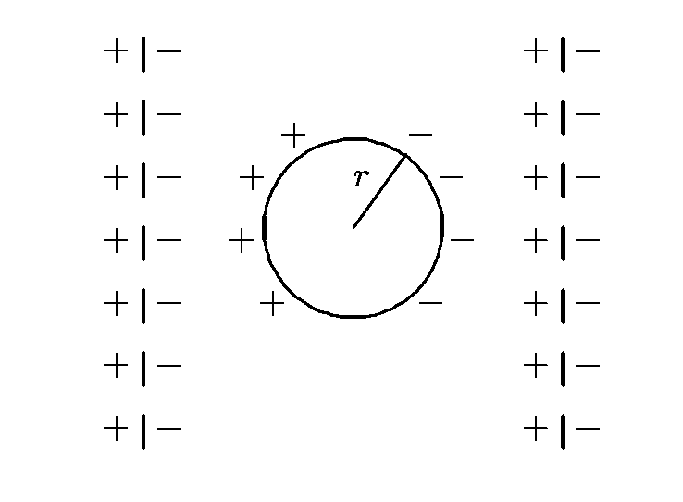
\includegraphics[scale=0.7]{Ris/ris_eps/ris2_01.eps}}}

\leftskip 0cm\centerline{\ris Рис. 2.1. К расчету внутреннего
поля.} \vskip 2mm Напряженность действующего на молекулу поля
может быть представлена суммой трех членов:
$$\vec F=\vec F_1+\vec F_2+\vec F_3.\noq$$
Здесь $\vec F_1$ --- поле, создаваемое обкладками конденсатора:
$$\vec F_1=\vec E+4\pi\vec P,$$
где $\vec P$ --- поляризация вещества. $\vec F_2$ --- поле,
обусловленное поляризацией вещества внутри конденсатора, за
вычетом вещества, находящегося внутри сферы. $\vec F_3$ --- поле,
создаваемое молекулами внутри сферы. Существенно, что сфера
мысленно проводится так, чтобы не пересекать ни одной молекулы:
каждая молекула, как целое, участвует в создании либо поля $\vec
F_2$, либо поля $\vec F_3$. Поле $\vec F_2$ в свою очередь состоит
из двух частей: из напряженности, создаваемой слоем зарядов,
индуцированных в диэлектрике у обкладок конденсатора:
$$\vec F'_{2}=-4\pi\vec P,$$
и напряженности поля $\vec F''_{2}$, создаваемого зарядами,
индуцированными на поверхности сферы:
$$\vec F_2=-4\pi\vec P+\vec F''_{2}.$$
Вычислим $\vec F''_{2}$. Плотность заряда на поверхности сферы
равна $p\cos\vartheta$, где $\vartheta$ --- угол между
положительным направлением поля и нормалью в данной точке сферы.
Каждый элемент поверхности сферы $d\Omega$ создает в направлении
поля напряженность, равную в центре сферы радиуса $r$
$${P_n\cos\vartheta\over r^2}d\Omega={P\cos^2\vartheta\over
r^2}d\Omega.$$ Интегрируя по поверхности всей сферы, находим:
$$F''_{2}=\int{P_n\cos\vartheta\over
r^2}d\Omega=\int\limits_0^{\pi}{P\cos^2\vartheta\over r^2}2\pi
r^2\sin\vartheta d\vartheta={4\pi\over3}P,$$ и, следовательно,
$$\vec F_2=-4\pi\vec P+{4\pi\over3}\vec P.$$
Остается вычислить поле $\vec F_3$, создаваемое молекулами,
находящимися внутри сферы. Считаем, что поле каждой молекулы есть
поле диполя. Потенциал в точке $x_0,y_0,z_0$, создаваемый диполем,
находящимся в точке $x,y,z$, отстоящей от $x_0,y_0,z_0$ на $r'$,
равен:
$$\varphi(x_0,y_0,z_0)={\vec p\vec {r'}\over
r'^3}={p_x(x_0-x)+p_y(y_0-y)+p_z(z_0-z)\over r'^3}.$$
Следовательно, в начале координат, в точке $x_0,y_0,z_0=0$ поле
имеет $x$-овую составляющую, равную
$$-\left(\partial\varphi\over\partial
x_0\right)_{x_0,y_0,z_0=0}=-{p_x\over r'^3}+{3\over r'^5}(p_xx^2+
p_yxy+p_zxz).$$ Считая, что диполи во всех молекулах одинаковы,
имеем:
$$\left(F_3\right)_x=p_x\left\{-\left.\sum_k\right.'{1\over
r'^3_k}+\left.\sum_k\right.'{3x_k^2\over
r'^5_k}\right\}+3p_y\left.\sum_k\right.'{x_ky_k\over
r'^5_k}+3p_z\left.\sum_k\right.'{x_kz_k\over r'^5_k}.$$
Суммирование распространяется на все молекулы, находящиеся внутри
сферы, за исключением находящейся в ее центре. При совершенно
хаотическом расположении диполей можем провести усреднение:
$$\left(F_3\right)_x=(N-1)=\left[p_x\left\{-\left({\overline{1}\over
r'^3}\right)+\left({\overline{3x^2}\over r'^5}\right)\right\}+p_y
\left({\overline{3xy}\over r'^5}\right)+p_z\left(
{\overline{3xz}\over r'^5}\right)\right].$$ Здесь $N$ --- число
молекул внутри сферы. Так как в изотропном теле
$\overline{x^2}=\overline{y^2}=\overline{z^2}={1\over3}\overline{r'^2}$;
$\overline{xy}=\overline{xz}=\overline{yz}=0$. Получаем $F_3=0$.

Аналогичный результат получается и для кристаллов, принадлежащих с
кубической системе --- оптически изотропных. Итак,
$$\vec F=\vec E+4\pi\vec P-4\pi\vec P+{4\pi\over3}\vec P=\vec
E+{4\pi\over3}\vec P.\noq$$ Мы пришли к этому результату,
рассматривая поведение вещества в электростатическом поле. Однако,
очевидно, что этот вывод в равной степени применим и к переменным
полям, в частности и к полю световой волны. Сопоставляя
соотношения \eqn{13} и
$$\vec D=\varepsilon\vec E=\vec E+4\pi\vec P,\noq$$
находим:
$$\vec F=\vec E+{4\pi\over3}{\varepsilon-1\over4\pi}\vec
E={\varepsilon+2\over3}\vec E={n^2+2\over3}\vec E.\noq$$ Это ---
выражение лорентцова внутреннего поля. Так как, с другой стороны,
$$\vec P=N_1\alpha\vec F,\noq$$
находим из \eqn{13-16}:
$${\varepsilon-1\over\varepsilon+2}={4\pi\over3}N_1\alpha,\noq$$
или
$${n^2-1\over n^2+2}={4\pi\over 3}N_1\alpha. \noq$$
Это соотношение называется формулой Лорентц-Лоренца.

\subzag{Молекулярная рефракция.} \vskip 2mm Формула Лорентц-Лоренца
\eqn{18} выражает зависимость показателя преломления $n$ от
плотности вещества --- от числа молекул в 1 ${\rm см^3}$ ($N_1$).
Разделив обе части уравнения \eqn{18} на плотность $\rho$ и
умножив их на молекулярный вес вещества, получим в правой части
уравнения величину, не зависящую от плотности, а значит, и от
температуры и давления. Имеем:
$${n^2-1\over
n^2+2}{M\over\rho}={M\over\rho}N_1{4\pi\over3}\alpha=N_A{4\pi\over3}\alpha=R,\noq$$
где $N_A=6,02\cdot10^{23}$ --- число Авогадро, равное числу
молекул в грамм-молекуле. Величина $R$ носит название {\it
молекулярной рефракции}. Ее размерность есть, очевидно,
размерность объема, и так как, в силу сказанного выше, $\alpha$
имеет порядок величины куба линейных размеров молекулы, $R$ должно
по порядку величины совпадать с объемом всех молекул в
грамм-молекуле, рассматриваемых в кинетической теории, как сферы.
Тем самым, порядок величины $R$ есть порядок кубических
сантиметров. Эти рассуждения приводят к выводу, что $R$ должно
совпадать с поправкой на объем в уравнении Ван-дер-Ваальса,
деленной на 4. Приводим некоторые данные (табл. 2.1). \vskip 1mm
\vbox{{\ris Таблица 2.1.}

\hskip 2cm\hbox{\vbox{\halign{\offinterlineskip \vrule\hskip
2mm\strut\hfil #\strut\hfil\hskip2mm &\vrule\hskip 2mm\strut\hfil
#\strut\hfil\hskip2mm &\vrule\hskip 2mm\strut\hfil
#\strut\hfil\hskip2mm &\vrule\hskip 2mm\strut\hfil
#\strut\hfil\hskip2mm &\vrule\hskip 2mm\strut\hfil
#\strut\hfil\hskip2mm & \vrule\hskip 2mm\strut\hfil
#\strut\hfil\hskip2mm & \vrule\hskip 2mm\strut\hfil
#\strut\hfil\hskip2mm &\vrule\hskip 2mm\strut\hfil
#\strut\hfil\hskip2mm \vrule\cr \noalign{\hrule} Вещество&${\rm
H_2}$&${\rm CS_2}$ &${\rm C_6H_{14}}$&${\rm C_6H_6}$&${\rm
H_2O}$&${\rm NH_3}$&${\rm C_6H_5Cl}$\cr\noalign{\hrule} $R,\ {\rm
см^{3}}$&2,0&21,7&29,7&25,9&3,7&5,6&31,1\cr\noalign{\hrule} \vbox
to 4mm {\vskip
0.5mm\hbox{${b\over4}$}}&5,0&19,5&44,0&37,0&7,7&9,5&36,1\cr\noalign{\hrule}
}}} }

Виду простоты и грубости исходных предположений, лучшего
совпадения ожидать не приходится. Независимость молекулярной
рефракции от давления иллюстрируется в табл. 2.2. \vskip 1mm
\vbox{{\ris Таблица 2.2.}

\hskip 2cm\hbox{\vbox{\halign{\vrule\hskip 2mm\strut\hfil
#\strut\hfil\hskip2mm &\vrule\hskip 2mm\strut\hfil
#\strut\hfil\hskip2mm &\vrule\hskip 2mm\strut\hfil
#\strut\hfil\hskip2mm \vrule\cr \noalign{\hrule} Давление,
атм.&$n$&$R,\ {\rm см^{3}}$\cr\noalign{\hrule}
1,00&1,0002929&2,170\cr 28,58&1,008385&2,170\cr
69,24&1,02044&2,180\cr 123,04&1,03633&2,175\cr
176,27&1,05213&2,170\cr\noalign{\hrule} }}} }

При очень высоких давлениях могут, однако, иметь место
значительные изменения $R$. Это объясняется изменением состояния
электронной оболочки молекулы и, следовательно, величины $\alpha$
в соответствующих условиях.

Практическая независимость молекулярной рефракции от температуры
подтверждается многочисленными опытами. Замечательным фактом
является относительная малость изменений $R$ при изменении
агрегатного состояния вещества, также следующая из формулы
\eqn{19}. Приводим некоторые данные (табл. 2.3).

А. И. Ансельм в своей теории показал, что эллипсоид поляризуемости
молекулы не изменяется при переходе из газа в конденсированную
фазу. Неизменна и оптическая анизотропия молекулы. Но вследствие
того, что в жидкостях существует корреляция в ориентациях
анизотропных молекул, меняются величины, зависящие от анизотропии
поляризуемости: степень деполяризации рассеянного света, константа
Керра и др. \vskip 1mm \vbox{{\ris Таблица 2.3.}

\hskip 2cm\hbox{\vbox{\halign{\vrule\hskip 2mm\strut\hfil
#\strut\hfil\hskip2mm &\vrule\hskip 2mm\strut\hfil
#\strut\hfil\hskip2mm &\hskip 2mm\strut\hfil #\strut\hfil\hskip2mm
&\vrule\hskip 2mm\strut\hfil #\strut\hfil\hskip2mm &\hskip
2mm\strut\hfil #\strut\hfil\hskip2mm \vrule\cr \noalign{\hrule}
Вещество&\omit\span\omit\vrule \hbox{\hskip 2mm Свойства
жидкости\hskip 2mm}&\omit\span\omit\vrule\hfill\hbox{\hskip 2mm
Свойства газа\hskip 2mm}\hfill\vrule\cr &$n$&$R,\ {\rm
см^{3}}$&$n$&$R,\ {\rm см^{3}}$\cr\noalign{\hrule} $\rm
Br_2$&1,659&9,45&1,000113&8,38\cr $\rm
O_2$&1,221&2,00&1,000271&2,01\cr $\rm
H_2$&1,10&0,92&1,000139&1,02\cr $\rm
N_2$&1,205&2,27&1,000296&2,193\cr $\rm
HCl$&1,245&6,88&1,000447&6,62\cr $\rm
H_2O$&1,334&3,71&1,000249&3,70\cr $\rm
NH_3$&1,325&5,55&1,000373&5,53\cr $\rm
SO_2$&1,410&11,67&1,000690&10,22\cr $\rm
CS_2$&1,628&21,34&1,00147&21,78\cr $\rm
CO_2$&1,192&6,80&1,000449&6,66\cr $\rm
CH_3OH$&1,3308&8,25&1,000549&8,14\cr $\rm
CHCl_3$&1,4467&21,42&1,001436&21,28\cr $\rm
C_2H_5OH$&1,3623&12,76&1,000871&12,92\cr\noalign{\hrule} }}} }

Все приведенные выше данные относятся к преломлению света с
длинной волны $\lambda=5890\angst$ ($D$-линия Na). Для других
волн, вследствие дисперсии, получатся иные значения $R$, но
практически независимые от плотности и агрегатного состояния
вещества.

Если вещество представляет собой смесь различных молекул, то
молекулярная рефракция смеси аддитивно складывается из рефракций
составляющих веществ.

Пусть в 1 $\rm см^{3}$ смеси содержится $N_1$ молекул первого
сорта, $N_2$ молекул второго сорта и т.д., общее число молекул в 1
$\rm см^{3}$ есть $N$:
$$N=N_1+N_2+...=N(f_1+f_2+...),\noq$$
причем величины
$$f_1={N_1\over N},\ f_2={N_2\over N},\cdots\ ,$$
характеризуют молярные концентрации компонент смеси. Плотность
смеси равна:
$$\rho={N\over N_A}\left(M_1f_1+M_2f_2+...\right)={\overline{M}\over
N_A}N,\noq$$ где $M_1,M_2,...$ --- молекулярные веса компонент
смеси, $\overline{M}$ --- средний молекулярный вес,
$M=M_1f_1+M_2f_2+...$\ . Из простых физических соображений
очевидно, что показатель преломления смеси должен выражаться
уравнением:
$${n^2-1\over
n^2+2}={4\pi\over3}(N_1\alpha_1+N_2\alpha_2+...),\noq$$ где
$\alpha_1,\alpha_2,...$ --- средние поляризуемости различных
веществ, входящих в состав смеси. Умножив \eqn{22} на
${\overline{M}\over \rho}={N_A\over N}$, получим среднюю рефракцию
смеси:
$$\overline{R}={n^2-1\over
n^2+2}{\overline{M}\over\rho}={4\pi\over 3}N_A(f_1\alpha_{1}+
f_2\alpha_2+...)=f_1R_1+f_2R_2+...\ ,\noq$$ что и требовалось
доказать.

Очевидно, что измерение показателя преломления дает возможность
анализа бинарных смесей на основе аддитивности рефракций.
Практически точность определения рефракции лимитируется
погрешностями измерения плотности, значительно более высокими, чем
погрешности при определении $n$. Так, например, при анализе смесей
вода-бензол, погрешность определения концентрации равна $0,008\%$,
для смеси вода-спирт --- $0,04\%$, вода-анилин --- $0,004\%$.
Особенно просты соотношения в случае газов, у которых $n$ близко к
единице. Имеем:
$$R\cong{2\over3}(n-1){M\over\rho}={2\over3}(n-1){N_AkT\over
p},\noq$$ где $k$ --- постоянная Больцмана, $p$ --- давление газа.
Для смеси газов получаем:
$$(n-1)p=(n_1-1)p_1+(n_2-1)p_2+...\ ,\noq$$
где $p_1,p_2,...$ --- парциальные давления. Одновременно
$$p=p_1+p_2+...\ .\noq$$
В случае смеси двух газов из этих уравнений следуют выражения для
объемных концентраций газов:
$${p_1\over p}={n_2-n\over n_2-n_1};\hskip 4mm{p_z\over
p}={n-n_1\over n_2-n_1}.\noq$$ Точность определения количества
$\rm CO_2$ в азоте, проведенного таким методом составляет 0,14\%.

\subzag{Аддитивность рефракций гомеополярных соединений.} \vskip
2mm Рефракция определенного вещества, и, следовательно, средняя
поляризуемость его молекул, может быть, в ряде случаев,
представлена в виде суммы рефракций, а значит и поляризуемостей
составных частей молекулы. В качестве таких составных частей можно
рассматривать образующие молекулу атомы, ионы или отдельные
валентные связи. Аддитивность имеет место не всегда, но во многих
случаях отклонения от нее незначительны. Этим объясняется большое
значение рефракции при определении структуры молекулы. Химические
свойства молекул определяются свойствами тех валентных связей,
которыми они образованы, и их относительным расположением. Исходя
из идеи аддитивности, получаем возможность зафиксировать те
существенные отклонения от аддитивности --- в частности от
аддитивности рефракций, которые представляют большой интерес,
характеризуя важные группы химических соединений.

Средняя поляризуемость молекулы выражает способность ее
электронной оболочки смещаться под действием внешнего
электрического поля. Электронная оболочка молекулы не может
считаться принадлежащей отдельным атомам. При образовании атомами
различных химических связей, за которые ответственны внешние
электроны, определяющие оптические свойства атомов и молекул,
поляризуемость их электронных оболочек существенно изменяет свой
характер. Так, не следует ожидать одинаковых рефракций у атомов
углерода, образующих единичные, двойные или тройные связи.

Для того, чтобы убедиться в аддитивности молекулярной рефракции,
сопоставим значения этой величины в гомологическом ряду
соединений, в котором каждый последующий член отличается от
предыдущего на одну и ту же группу атомов. Если аддитивность
рефракций действительно имеет место, то разности рефракций любых
двух следующих друг за другом членов ряда должны быть одинаковыми.
Приводим данные для предельных углеводородов нормального строения
(табл. 2.4). \vskip 1mm \vbox{{\ris Таблица 2.4.}

\hskip 2cm\hbox{\vbox{\halign{\vrule\hskip 2mm\strut\hfil
#\strut\hfil\hskip2mm &\vrule\hskip 2mm\strut\hfil
#\strut\hfil\hskip2mm &\vrule\hskip 2mm\strut\hfil
#\strut\hfil\hskip2mm &\vrule\hskip 2mm\strut\hfil
#\strut\hfil\hskip2mm \vrule\cr \noalign{\hrule}
Вещество&Формула&$R,\ {\rm см^{3}}$&$\Delta R, {\rm
см^{3}}$\cr\noalign{\hrule} н-пентан&$\rm
H_3C-CH_2-CH_2-CH_2-CH_3$&25,28&$-$\cr н-гексан&$\rm
H_3C-(CH_2)_4-CH_3$&29,86&4,58\cr н-гептан&$\rm
H_3C-(CH_2)_5-CH_3$&34,51&4,65\cr н-октан&$\rm
H_3C-(CH_2)_6-CH_3$&39,13&4,62\cr н-нонан&$\rm
H_3C-(CH_2)_7-CH_3$&43,78&4,65\cr н-декан&$\rm
H_3C-(CH_2)_8-CH_3$&48,41&4,63\cr н-ундекан&$\rm
H_3C-(CH_2)_9-CH_3$&53,06&4,65\cr н-додекан&$\rm
H_3C-(CH_2)_{10}-CH_3$&57,67&4,61\cr\noalign{\hrule} }}} }

Аддитивность действительно имеет место. У изомерных ---
разветвленных предельных углеводородов рефракции не отличаются от
рефракций соответствующих соединений нормального строения. Можно
представить рефракцию предельного углеводорода $\rm C_nH_{2n+2}$ в
виде:
$$R_{C_nH_{2n+2}}=nR_C+(2n+2)R_H.$$
Значит, средняя разность $\Delta R=4,618$, приходящаяся на одну
группу $\rm CH_2$, может быть представлена как
$$4,618=R_C+2R_H.$$
Сопоставляя значение рефракции предельных углеводородов, находим
<< рефракцию углерода>>\ и << рефракцию водорода>>:
$$R_C=2,418{\rm см^{3}}\hskip 4mm;R_H=1,100{\rm см^{3}}.$$
Однако для того же атома углерода, но входящего в состав
непредельного соединения и образующего двойную связь, приходится
вводить другую величину:
$$R_{C=}=4,151 {\rm см^{3}}.$$
Принято говорить, что $R_{C=}$ (или $R_C$ в соединениях
ацетиленового ряда) отличается от $R_{C\equiv}$ на величину так
называемого инкремента, инкременты для двойной и тройной связи
обозначаются соответственно значками \inkdu и \inktri. Они имеют
значения:
$$\inkdu=1,733 {\rm см^{3}}\hskip 4mm\inktri=2,398 {\rm см^{3}}.$$
Таким образом,
$$R_{C=}=R_c+\inkdu=2,418+1,733=4,151;$$
$$R_{c\equiv}=R_C+\inktri=2,418+2,398=4,816.$$
Таким образом, рефракция молекулы представляется формулой:
$$R=\sum_nR_n+\sum_iI_i,\noq$$
где первая сумма есть сумма рефракций атомов, а вторая --- сумма
необходимых инкрементов. Введение этих последних свидетельствует о
формальности схемы атомных рефракций. Разложение рефракции по
валентным связям физически более обосновано, так как
поляризующиеся электроны локализованы именно на отдельных
валентных связях, образуя их, но не могут быть приписаны отдельным
атомам. При таком разложении необходимость вводить инкременты
отпадает, и выражение молекулярной рефракции представляется в
виде:
$$R=\sum_kR_k,\noq$$
где $R_k$ --- рефракция отдельной связи, и суммирование
распространяется по всем связям в молекуле. Но разложение \eqn{28}
применяется чаще. Формально это приемлемо, так как при наличии
аддитивности \eqn{29} можно с помощью инкрементов установить
однозначное соответствие между атомарными рефракциями и
рефракциями связей. Очевидно, например, что поскольку углерод в
насыщенных соединениях образует четыре валентных связи $\rm C-H$
или четыре валентных связи $\rm C-C$, должно иметь место
соотношение:
\begin{plain}$$\eqalign{R_{C-H}=&{1\over4}R_C+R_H,\cr
R_{C-C}=&{1\over4}R_C+{1\over4}R_C={1\over2}R_C }.$$ \end{plain} Для кратных
связей имеем:
$$R_{C=C}={1\over2}R_C+{1\over2}R_C+\inkdu=R_C+\inkdu,$$
$$R_{C\equiv C}={3\over2}R_C+\inktri,$$
и наоборот:
\begin{plain}$$\eqalign{
R_C=&2R_{C-C},\cr R_H=&R_{C-H}-{1\over2}R_{C-C},}$$
$$\inkdu=R_{C=C}-2R_{C-C},$$
$$\inktri=R_{C\equiv C}-3R_{C-C}.$$
\end{plain}
Значения рефракций атомов и групп с указанием этих величин для
разных длин волн приведены в таблице 7, страница 60 книги <<
Молекулярная оптика>>\ М. В. Волькенштейна. Данные в ней получены
путем сопоставления молекулярных рефракций ряда соединений на
основе аддитивности. Пользуясь данными этой таблицы и ранее
написанными соотношениями, находим:
\begin{plain}$$\eqalign{
R_{C-H}=&1,705;\cr R_{C-C}=&1,209;\cr R_{C=C}=&4,151;\cr
R_{C\equiv C}=&6,025. }$$\end{plain} Все величины для $D$-линии Na. Приведем
таблицу рефракций связей (табл. 2.5). \vskip 1mm \vbox{{\ris
Таблица 2.5.}

\hskip 2cm\hbox{\vbox{\halign{\vrule\hskip 2mm\strut\hfil
#\strut\hfil\hskip2mm &\vrule\hskip 2mm\strut
#\strut\hfil\hskip2mm &\vrule\hskip 2mm\strut\hfil
#\strut\hfil\hskip2mm \vrule\cr \noalign{\hrule} Связь&&$R,\ {\rm
см^{3}}$, D-линия Na\cr\noalign{\hrule} $\rm C-H$&&1,676\cr $\rm
C-C$&&1,296\cr $\rm C=C$&&4,17\cr $\rm C\equiv C$&на конце
цепи&5,87\cr $\rm C\equiv C$&в середине цепи&6,24\cr $\rm C-C$&в
циклопропане&1,49\cr $\rm C-C$&в циклобутане&1,37\cr $\rm C-C$&в
циклопентане&1,26\cr $\rm C-C$&в циклогексане&1,27\cr $\rm C-C$&в
ароматических соединениях&2,688\cr $\rm C-F$&&1,44\cr $\rm
C-Cl$&&6,51\cr $\rm C-J$&&14,61\cr $\rm C-O$&в эфирах&1,54\cr $\rm
C=O$&в метилкетонах&3,49\cr $\rm C-N$&&1,57\cr $\rm C=N$&&3,76\cr
$\rm C\equiv N$&&4,82\cr\noalign{\hrule} }}} }

\subzag{Рефракция неаддитивных соединений.} \vskip 2mm Для
некоторых групп органических соединений характерно отклонение от
аддитивности рефракций (экзальтация рефракции). В первую очередь
это относится к веществам, содержащим сопряженные двойные связи и
ароматическими соединениями.

Простейшим веществом с сопряженными двойными связями является
бутадиен (дивинил): $\rm H_2C=CH-CH=CH_2$. Его рефракция превышает
вычисленную по аддитивной схеме на $1,42 \rm см^{3}$. Эта величина
носит название экзальтации рефракции:
$$\Delta R=R-\sum_kR_k.\noq$$
Как показывает опыт, экзальтация рефракции тем выше, чем больше
сопряженных связей или ароматических ядер в молекуле содержится.
Понижение симметрии молекулы --- введение метильной группы в
боковую цепочку --- понижает экзальтацию. Например:
\begin{plain}$$\eqalign{
&\hbox{для}\ {\rm H_2C=CH-CH=CH_2}\hskip 4mm \hbox{---}\ \Delta
R=1,42;\cr &\hbox{для}\ {\rm H_2C=\vbox{\hbox{$\rm CH_3$}\vskip
-9.7mm\hbox{$\hskip 1mm |$}\vskip -9mm\hbox{$\rm C$}}\hskip -4mm
-CH=CH_2}\hskip 6.5mm \hbox{---}\ \Delta R=0,88. }$$\end{plain} До сих пор не
имеет объяснения факт отсутствия экзальтации у бензола и некоторых
сходных соединений при одновременном большом значении экзальтации
нафталина и последующих членов ряда ароматических соединений:

\vskip 3mm
\centerline{\hbox{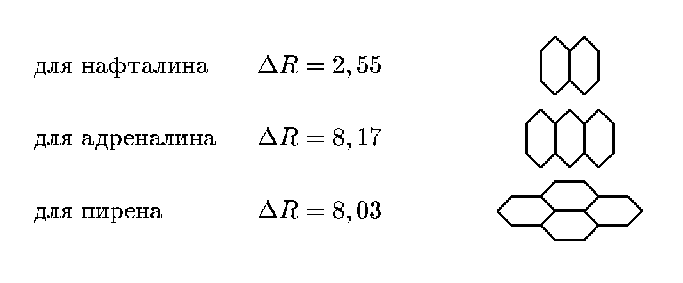
\includegraphics[scale=0.7]{Ris/ris_eps/ris2_01a.eps}}}

\leftskip 0cm Экзальтация может достигать весьма высоких значений,
составляющих существенную долю общей рефракции вещества. Например,
для молекулы мезо-тетрафенилпорфирина $ R=293 \rm см^{3}$, $\Delta
R=90 \rm см^{3}$.

Объяснение этим фактам нужно искать в строении рассматриваемых
молекул. Такие факторы, как сопряжение двойных связей, приводят к
делокализации, обобществлению электронов между связями. В этих
случаях теряет смысл выделение отдельной связи как аддитивной
структурной единицы --- электронная оболочка принадлежит группе
связей или даже всей молекуле. С особенной яркостью эти
обстоятельства проявляются в электронных спектрах поглощения и в
спектрах комбинационного рассеяния.

\subzag{Рефракция ионных соединений.} \vskip 2mm Для ряда молекул,
которые могут считаться в первом приближении построенными из
ионов, также имеет место аддитивность. Ионные соединения
представляем себе в виде раздельных положительного и
отрицательного ионов, удерживаемых друг около друга на
определенном расстоянии кулоновскими электростатическими силами
притяжения и силами отталкивания. Поэтому следует считать разумным
разложение рефракции ионной молекулы на рефракции ионов.

Однако аддитивность в ионных соединениях соблюдается не строго.
Поляризующиеся электронные оболочки соседних ионов
взаимодействуют. В частности, протон, благодаря своему малому
размеру --- отсутствию внешних электронов --- глубоко проникает в
электронную оболочку аниона и сильно изменяет поляризуемость
последнего, уменьшая ее.

Сопоставим рефракции следующих изоэлектронных соединений: \vskip
1mm \hfil\hbox{\vbox{\halign{\vrule\hskip 2mm\strut\hfil
#\strut\hfil\hskip2mm &\hskip 2mm\strut\hfil #\strut\hfil\hskip2mm
&\vrule\hskip 2mm\strut\hfil #\strut\hfil\hskip2mm &\hskip
2mm\strut\hfil #\strut\hfil\hskip2mm \vrule\cr \noalign{\hrule}
$\rm Cl^-$&9,30&HCl&6,67\cr $Br^-$&12,04&HBr&9,19\cr
$J^-$&19,07&HJ&13,74\cr\noalign{\hrule} }}}\hfill

Упрощенные электростатические представления вынуждают вводить при
расчете рефракции неорганических соединений различные поправки на
взаимодействие ионов между собой и на влияние окружающей среды.
Например, рефракция иона $\rm Cl^-$, определяемая из соединений
$\rm NaCl$, $\rm MgCl_2$, $\rm AlCl_3$, $\rm SiCl_4$, $\rm PCl_5$,
различна не вследствие различий во взаимной поляризации, которые
могут быть учтены простым электростатическим расчетом. В
действительности, в указанном ряду меняется характер химической
связи, становящейся при переходе слева направо все более
гомеополярной.

Из всего вышеизложенного следует, что схема аддитивности ионных
рефракций применима только как первое приближение, полезное для
целей предварительной ориентировки.

\subzag{Определение показателя преломления методом предельного
угла.} \vskip 2mm Если луч света пересекает границу раздела двух
прозрачных однородных сред 1 и 2 (рис. 2.2), то направление луча
изменяется в соответствии с установленным еще в начале XVII века
законом преломления. Согласно этому закону, отношение синусов
углов падения $i_1$ и преломления $i_2$ есть величина постоянная:
$${\sin i_1\over\sin i_2}=n_{12}.\noq$$

\vskip 3mm
\centerline{\hbox{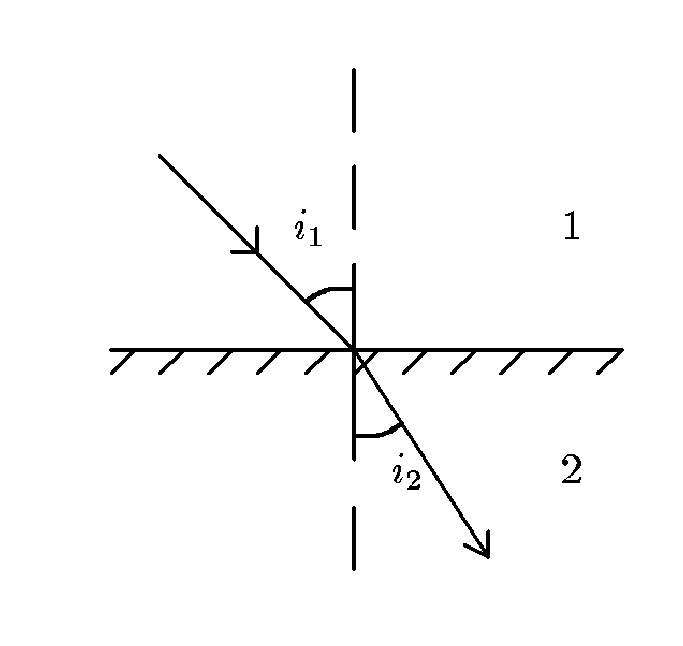
\includegraphics[scale=0.7]{Ris/ris_eps/ris2_02.eps}}}

\leftskip 0cm \centerline{\ris Рис. 2.2. Преломление луча на
границе двух прозрачных сред.} \vskip 2mm Константа $n_{12}$
называется относительным показателем (или коэффициентом)
преломления второго вещества по отношению к первому.

Волновая теория света устанавливает простую связь показателя
преломления со скоростью распространения световых волн в двух
средах $v_1$ и $v_2$:
$$n_{12}={v_1\over v_2}.\noq$$
Показатель преломления по отношению к << пустоте>>\ называется
абсолютным показателем преломления. Из формулы \eqn{32} следует,
что абсолютный показатель преломления вещества $n$ равен отношению
скорости света в пустоте $c=3\cdot10^{10}$ см/сек к скорости света
в веществе $v$:
$$n={c\over v}.\noq$$
Относительный показатель преломления $n_{12}$ согласно \eqn{32} и
\eqn{33}, равен отношению абсолютных показателей преломления
веществ 1 и 2:
$$n_{12}={n_2\over n_1}.\noq$$
Принимая во внимание это соотношение, закон преломления \eqn{31}
можно записать в удобной для запоминания форме:
$$n_1\sin i_1=n_2\sin i_2.$$

При измерении показателей преломления жидких и твердых тел обычно
определяются их относительные показатели преломления по отношению
к воздуху лабораторного помещения.

Показатели преломления по отношению к воздуху в химической
рефрактометрии просто называют показателями преломления и
обозначают буквой $n$. Абсолютные показатели преломления
обозначают {\bfseries n}. Соотношение между {\bfseries n} и $n$,
согласно определению этих величин и формуле \eqn{34}, следующее:
$$\hbox{\bfseries n}=\hbox{\bfseries n}_{\rm воздуха}\cdot n.\noq$$
Таким образом, для получения абсолютных показателей преломления
достаточно умножить определяемые при обычных рефрактометрических
измерениях величины на абсолютный показатель преломления воздуха.

При нормальном атмосферном давлении и комнатной температуре
$\hbox{\bfseries n}_{\rm воздуха}=1,00027$, следовательно:
$$\hbox{\bfseries n}=1,00027\cdot n.\noq$$
Соотношение \eqn{36} --- приближенное, так как не учитывает
зависимости абсолютного показателя преломления воздуха от
давления, температуры и влажности. В подавляющем большинстве
случаев, когда не требуется абсолютной точности измерения n,
превышающей $1\cdot10^{-4}$, такое упрощение вполне допустимо.

Показатель преломления вещества определяется его природой, но
зависит также от внешних условий (главным образом от температуры и
от длины волны света). Длину волны указывают подстрочным индексом,
а температуру --- надстрочным индексом справа. Например, символ
$n_{480}^{25}$ обозначает показатель преломления при 25$^{\circ}$C
для голубой линии кадмия с длиной волны 480 нм ($4800 \angst$).
Вместо длины волны часто употребляемых спектральных линий обычно
указывают их буквенные обозначения. Так, например, $n_{D}^{20}$,
$n_C^{20}$ и $n_F^{20}$ обозначают показатели преломления при
20$^{\circ}$C для линии $D$ натрия (5893\angst) и линий $C$ и $F$
водорода ($\lambda_C=6563\angst,\ \lambda_F=4861\angst$).

У оптически анизотропных веществ, к которым относится большинство
кристаллов (кроме кристаллов кубической системы), наблюдается
двойное лучепреломление --- расщепление преломляющегося луча на
два луча, распространяющихся с разными скоростями. При этом у так
называемых одноосных кристаллов (гексагональной, тетрагональной и
тригональной систем) скорость распространения одного из лучей,
называемого необыкновенным, зависит от его направления. В
оптически двуосных кристаллах низкой симметрии (ромбической,
моноклинной и триклинной систем) скорость распространения обоих
преломленных лучей зависит от направления. В связи с этим
оптически анизотропные вещества характеризуются двумя
экстремальными показателями $n_{o}$ и $n_{e}$ (одноосные
кристаллы) или тремя показателями $n_p,n_m,n_g$ (двуосные
кристаллы). В данном случае индексы $o$ и $e$ относятся к
обыкновенному и необыкновенному лучам, а индексы $p,\ g$ и $m$
обозначают соответственно наименьший, наибольший и промежуточный
показатели преломления в трех взаимно перпендикулярных
направлениях.

Согласно закону преломления света \eqn{31}, при $n_{12}={n_2\over
n_1}>1$, $\sin i_1>\sin i_2$, и, следовательно, $i_1>i_2$. Отсюда
следует, что при преломлении света угол $i_2$ не может быть больше
некоторой величины $\varphi<90^{\circ}$, соответствующей
$i_1=90^{\circ}$ и определяемой непосредственно вытекающим из
закона преломления соотношением:
$$\sin\varphi={n_1\over n_2}.\noq$$
Как показывает опыт, луч, падающий из среды с большим показателем
преломления на границу раздела с менее преломляющей средой под
углом $i_2>\varphi$, не преломляется, а полностью отражается (рис.
2.3). Это явление, называемое полным внутренним отражением, было
известно давно и отмечено Кеплером еще до открытия закона
преломления света.

\vskip 3mm
\centerline{\hbox{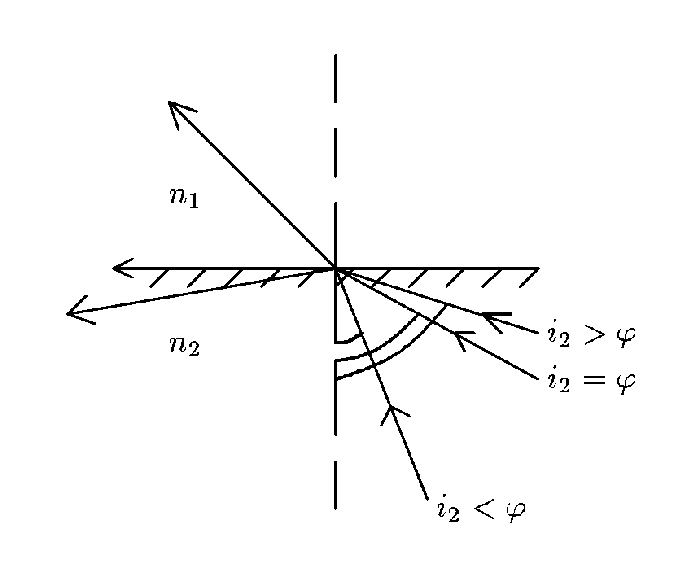
\includegraphics[scale=0.7]{Ris/ris_eps/ris2_03.eps}}}

\leftskip 0cm\centerline{\ris Рис. 2.3. Полное внутреннее
отражение.} \vskip 0.5mm \noindent{\Small Лучи, падающие на границу
раздела из более преломляющей среды (${\mitsm n_1<n_2}$) под
углом, превышающим ${\mitsm\varphi}$ (предельный угол), полностью
отражаются от границы раздела.} \vskip 2mm При $i_2<\varphi$
происходит преломление луча, сопровождающееся частичным отражением
от границы раздела. Предельное значение $i_2=\varphi$ называется
предельным, или критическим углом.

Предельный угол можно измерять двумя способами. Во-первых, можно
направить на границу раздела пучок лучей со стороны среды с
большим показателем преломления под углом, близким к предельному,
и наблюдать отраженный свет, как показано на рис. 2.4а. Во-вторых,
можно осветить границу раздела сред скользящим пучком лучей со
стороны слабопреломляющей среды и рассматривать преломленные лучи
(рис. 2.4б). В обоих случаях наблюдается граница светотени,
соответствующая предельному углу. Второй способ (способ <<
скользящего вхождения лучей>>\ или способ << работы в проходящем
свете>>) дает очень отчетливую и контрастную границу, но пригоден
только для прозрачных сред. Первый из этих способов (работа в
отраженном свете) может применяться и в том случае, когда
слабопреломляющая среда малопрозрачна, но дает небольшую разницу
освещенностей светлой и затемненной частей поля зрения, так что
граница наблюдается труднее.

Для наблюдения предельного угла на плоской границе между двумя
твердыми телами необходимо устранить тончайшую прослойку воздуха,
которая остается между полированными поверхностями твердых тел при
простом наложении их друг на друга. Устранения воздушной прослойки
достигают, раздавливая между складываемыми гранями каплю жидкости
с высоким показателем преломления, так называемой контактной
жидкости. Показатель преломления контактной жидкости должен быть
больше, чем у твердого тела, в противном случае наблюдаемый
предельный угол будет соответствовать полному внутреннему
отражению на границе жидкости и твердого тела, а не на границе
двух твердых тел.

\vskip 3mm
\centerline{\hbox{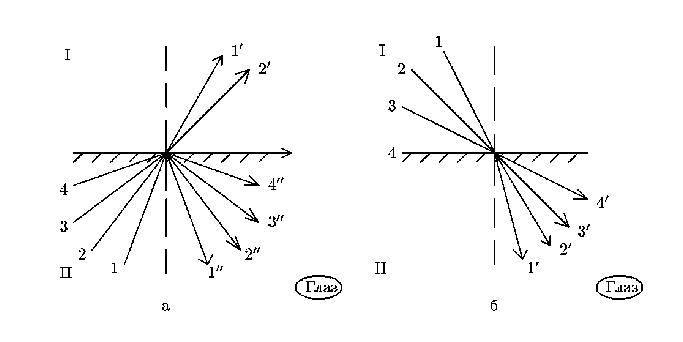
\includegraphics[scale=0.7]{Ris/ris_eps/ris2_04.eps}}}

\leftskip 0cm\centerline{\ris Рис. 2.4. Два способа наблюдения
предельного угла.}

\noindent{\Small а --- в отраженном свете, б --- в проходящем
свете. I --- среда с меньшим показателем преломления; II --- среда
с большим показателем преломления.} \vskip 2mm Непосредственный
оптический контакт между поверхностями двух твердых тел может быть
достигнут, если одна из этих поверхностей плоская, а другая слабо
выпуклая. При сдавливании таких поверхностей возникают кольца
Ньютона, причем на центральном пятне можно наблюдать полное
внутреннее отражение без контактной жидкости. Такой метод
наблюдения полного внутреннего отражения может быть полезен при
измерении показателей преломления сильнопреломляющих твердых тел,
когда трудно подыскать контактную жидкость с достаточно высоким
показателем преломления.

Величина предельного угла на границе двух веществ зависит только
от показателей преломления этих веществ. Следовательно, если
известен показатель преломления одного вещества, то показатель
преломления другого вещества можно определить, измерив предельный
угол $\varphi$:
$$n_1=n_2\sin\varphi.\noq$$
Удобство этого способа состоит в том, что требуется измерение
только одного угла, а исследуемому телу не надо придавать строго
определенную геометрическую форму, так как для наблюдения полного
внутреннего отражения существенно лишь наличие плоской границы
раздела.

Измерение предельного угла для определения показателей преломления
было, по видимому, впервые использовано Волластоном в начале XIX
в. С конца XIX в., когда были созданы удобные конструкции
специальных рефрактометров, метод предельного угла получил широкое
распространение и в настоящее время служит важнейшим способом
измерения показателей преломления в химических приложениях
рефрактометрии.

Существенной деталью большинства рефрактометров, основанных на
определении предельного угла, является измерительная призма из
оптического стекла с точно известным показателем преломления N.
Одна из граней измерительной призмы (так называемая входная грань)
приводится в оптический контакт с измеряемым телом и служит
границей раздела, на которой происходит преломление и полное
внутреннее отражение. Преломление или отражение света на этой
грани наблюдается в зрительную трубу обычно через вторую
(выходную) грань призмы (рис. 2.5).

\vskip 3mm
\centerline{\hbox{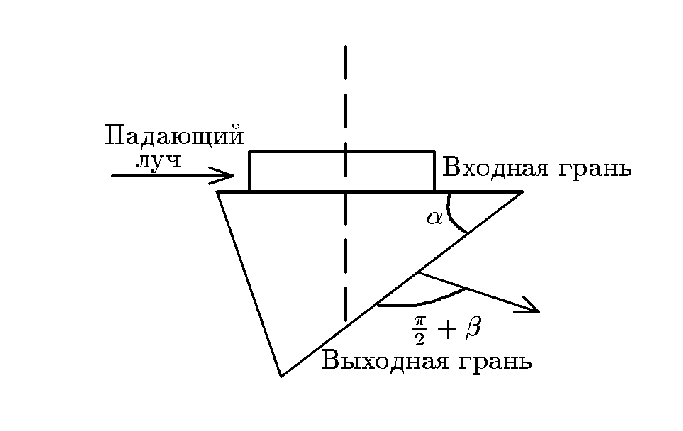
\includegraphics[scale=0.7]{Ris/ris_eps/ris2_05.eps}}}

\leftskip 0cm\centerline{\ris Рис. 2.5. Принципиальная схема
рефрактометра, основанного на измерении предельного угла.} \vskip
2mm Как сказано выше, угол $\alpha$ между входной и выходной
гранями называется преломляющим углом призмы. Луч, соответствующий
предельному углу $\varphi$ и называемый предельным лучом, после
преломления на границе стекло призмы --- воздух составляет с
нормалью к выходной грани некоторый угол $\beta$.

При рассматривании вышедших из призмы лучей, близких к
предельному, поле зрения трубы оказывается разделенным на
освещенную и темную части, граница между которыми соответствует
предельному лучу.

Разные типы рефрактометров предельного угла отличаются величиной
преломляющего угла измерительных призм, величиной их показателей
преломления, конструкцией угломерных устройств и применяемыми
источниками света.

Каждый рефрактометр предельного луча пригоден для измерения
показателей преломления только в определенных пределах их значений
и в этом отношении не является прибором вполне универсальным.
Верхний предел измеряемых показателей преломления $n$ зависит от
показателя преломления стекла измерительной призмы $N$. Нетрудно
видеть, что при показанном на рис. 2.5 способе наблюдения
предельного луча должно соблюдаться неравенство $n<N$, т.е.
измеряемый показатель преломления должен быть меньше показателя
преломления призмы. Нижний предел измеряемых $n$ зависит от
конструкции прибора (угла $\alpha$, размеров призм, угломерного
устройства).

Как следует из изложенного, в методе предельного угла измеряется
обычно не непосредственно предельный угол $\varphi$, а угол
$\beta$ между предельным лучом и нормалью к выходной грани.

Формулу, связывающую величину угла $\beta$ с показателем
преломления исследуемого вещества $n$, нетрудно получить,
рассматривая преломление предельного луча на гранях призмы. Для
полного внутреннего отражения на входной грани имеем соотношение:
$$\sin\varphi={n\over N},\noq$$
а для преломления на выходной грани:
$$\sin\beta=N\sin\beta',\noq$$
причем
$$\beta'=\pm(\varphi-\alpha)\ \ \hbox{или}\ \
\varphi=\alpha\pm\beta'.\noq$$ Знак << плюс>>\ в уравнениях
\eqn{34} относится к случаю, когда предельный луч выходит от
нормали в сторону преломляющего ребра призмы, как на рис. 2.5, а
знак << минус>>\ --- когда предельный луч располагается по
другую сторону нормали. Исключая промежуточные углы $\beta'$ и
$\varphi$ из уравнений \eqn{39-41}, получим:
$$n=\sin\alpha\left(\sqrt{N^2-\sin^2\beta}\right)\pm\cos\alpha\sin\beta.\noq$$
Эта формула лежит в основе всех расчетов при измерениях методом
предельного угла на призме. По формуле \eqn{42} производятся
вычисления показателей преломления $n$, расчеты шкал
рефрактометров и вспомогательных таблиц к ним.

Дифференцируя \eqn{42} по $N$, $\alpha$ или $\beta$, нетрудно
получить соотношения, необходимые для учета возможных погрешностей
измерений. Наиболее важным из них является соотношение для учета
несоответствия истинного значения показателя преломления стекла
призмы принимаемому при расчете значению $N$. Ошибка $\Delta N$
повлечет за собой ошибку в определении $n$, равную:
$$\Delta n={N\sin\alpha\over\sqrt{N^2-\sin^2\beta}}\Delta N.\noq$$
Формула \eqn{43} используется, в частности, для внесения
температурных поправок, когда $\Delta N$ вызывается отклонением
температуры призмы от стандартной.

Неточность преломляющего угла призмы $\Delta \alpha$ вызовет
ошибку измерения показателя преломления $\Delta n$:
$$\Delta
n=\left(\cos\alpha\left(\sqrt{N^2-\sin^2\beta}\right)-\sin\beta\sin\alpha
\right)\Delta\alpha=\left(\sqrt{N^2-n^2}\right)\Delta\alpha.\noq$$
Наконец, угломерная ошибка $\Delta\beta$ приведет к ошибке $\Delta
n$, равной:
$$\Delta
n={\cos^2\beta\sqrt{N^2-n^2}\over\sqrt{N^2-\sin^2\beta}}\Delta\beta.\noq$$

\subzag{Рефрактометры типа Пульфриха. ИРФ-23.} \vskip 2mm
Рефрактометр Пульфриха --- основной прибор, применяемый для
специальных исследовательских работ в области химических
приложений рефрактометрии.

Характерной особенность рефрактометров Пульфриха является
использование источников света с линейчатым спектром и
измерительных призм с преломляющим углом 90$^{\circ}$. Принцип
действия прибора основан на явлениях, происходящих при прохождении
света через границу раздела двух сред с разными показателями
преломления. Подставив $\alpha=90^{\circ}$ в основную формулу,
получим формулу для определения показателя преломления на
рефрактометрах данного типа:
$$n=\sqrt{N^2-\sin^2\beta}.\noq$$
если скользящий луч, падающий из среды с меньшим показателем
преломления $n$, отклонить до предела и пустить вдоль поверхности
второй среды под углом $90^{\circ}$ с нормалью, то во второй среде
с большим показателем преломления $N$ он выйдет под углом $\beta$.
Ход лучей в призме рефрактометра Пульфриха схематически показан на
рис. 2.6.

\vskip 3mm
\centerline{\hbox{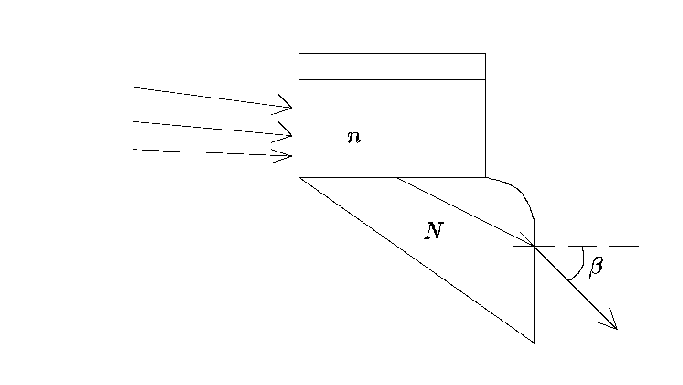
\includegraphics[scale=0.7]{Ris/ris_eps/ris2_06.eps}}}

\leftskip 0cm\centerline{\ris Рис. 2.6. Ход лучей в измерительной
призме рефрактометра Пульфриха.} \vskip 2mm Рефрактометр снабжен
набором измерительных призм, из которых всегда можно выбрать
призму с показателем преломления большим, чем у измеряемого
вещества.

На приборе определяются показатели преломления прозрачных жидких и
твердых веществ. В первом случае исследуемая жидкость наливается в
стаканчик, который предварительно приклеивается к измерительной
призме прибора. Конструктивно измерительная призма выполнена так,
что место склейки ее со стаканчиком находится ниже ее верхней
грани и не мешает прохождению лучей. Края верхней грани призмы
сошлифованы по сфере, так что входная грань имеет форму круга,
радиус которого несколько меньше внутреннего радиуса стаканчика.
Нижняя часть стаканчика также имеет сферический шлиф, притертый по
сферической части призмы.

При испытании твердых тел исследуемый образец, имеющий две плоские
полированные поверхности, расположенные под прямым углом,
накладывается на верхнюю грань измерительной призмы. При этом
между соприкасающимися поверхностями образца и призмы помещается
тонкий слой (одна капля) жидкости с показателем преломления,
превышающим показатель преломления исследуемого образца, но не
превышающим показатель преломления измерительной призмы.

Устройство для измерения угла $\beta$ состоит из зрительной трубы,
наглухо соединенной со стеклянным лимбом, закрытым металлическим
кожухом, и спирального микрометра. В окуляре микрометра имеется
вертикальная шкала с десятью делениями, каждое из которых
соответствует 0,1$^{\circ}$. Сотые и тысячные доли градуса
определяются при помощи вращающейся спирали с двойными витками.
Шаг этой спирали (смещение при полном обороте) точно равен
расстоянию между делениями окулярной шкалы, т.е. соответствует
$0,001^{\circ}$. Маховичком вращают спираль до тех пор, пока
градусный штрих лимба не расположится симметрично между двойными
штрихами витка спирали. Номер этого градусного штриха дает число
целых градусов. Десятые доли определяются числом целых делений
окулярной шкалы, пройденных градусным штрихом лимба. Сотые и
тысячные доли отсчитывают против индекса на кольцевой шкале
спирали.

Таким образом, точность и удобство измерений углов значительно
повышаются и отпадает необходимость в отдельной шкале
микрометрического винта для дифференциальных измерений.
Микрометрический винт служит в приборе только для точной наводки
трубы.

В фокальной плоскости окуляра трубы расположен визирный крест,
наводимый при измерениях на границу внутреннего отражения. При
рассматривании границы полного внутреннего отражения в трубу
наблюдается ряд спектральных полос, ширина которых зависит от
положения диафрагмы конденсатора, ограничивающей сверху пучок
падающих на призму лучей. Поворотом диафрагмы можно регулировать
ширину полос и добиться разделения близко расположенных
спектральных линий.

Взаимное расположение спектральных полос зависит от соотношения
численных значений дисперсий измеряемого вещества и стекла призмы.
Чем больше они различаются, тем больше видимое расстояние между
полосами. Обычно дисперсия измеряемого вещества меньше дисперсии
стекла призмы, и вверху поля зрения располагаются красные линии, а
внизу --- синие и фиолетовые. Обратное (необычное) расположение
линий имеет место, когда дисперсия вещества больше дисперсии
призмы. Чтобы измерить угол $\beta$, надо навести крест на верхнюю
(резкую) границу спектральной полосы и произвести отсчет по лимбу
и спиральному микрометру. Распространенной ошибкой является
установка креста не на верхнюю границу, а на середину спектральной
полосы. Ширина спектральной полосы, а следовательно, и положение
ее середины зависит от положения диафрагмы конденсатора.
Результаты измерений при такой неправильной установке креста будут
ниже истинных значений показателей преломления. К рефрактометру
Пульфриха прилагается несколько призм, каждая из которых
предназначается для измерений в определенных пределах $n$. Полный
комплект к прибору ИРФ-23 состоит из трех призм. Призма № 1
изготавливается из флинта Ф-2 ($N_D=1,617$) и предназначена для
работы с жидкими и твердыми образцами, имеющими $n=1,31\div 1,61$.
Призма № 2 сделана из тяжелого флинта ТФ-4 ($N_D=1,740$) и
позволяет измерять $n=1,46\div 1,73$. Призма № 3 делается из
стекла ТФ-10 с очень высоким показателем преломления ($N_D=1,806$
и служит для измерения $n$ некоторых сильно преломляющих стекол и
неорганических жидкостей, не укладывающихся в интервал показателей
призмы № 2 ($n=1,54\div 1,80$).

К каждой призме имеется таблица для перевода углов $\beta$ в
показатели преломления, рассчитанная по формуле \eqn{46}. Точные
значения показателей преломления призм, изготовленных в разное
время из стекла разных варок, несколько различаются и гравируются
на матовой части верхней поверхности призм. Следует обращать
внимание на соответствие указанных в таблицах значений показателей
преломления выгравированным на самих призмах.

\subzag{Интерференционно-поляризационный метод измерения разности
показателей преломления.} \vskip 2mm Сущность
интерференционно-поляризационного метода измерения разности
показателей преломления заключается в поляриметрическом
определении разности хода двух лучей со взаимно ортогональными
плоскостями поляризации, интерферирующими после прохождения через
среды с показателями преломления $n_1$ и $n_2$.

Академик Лебедев одним из первых практически применил схему
поляризационного интерферометра для определения под микроскопом
показателя преломления микроскопических зерен и оптических
неоднородностей в оптических стеклах, а также в тонких
биологических срезах. Затем модификация схемы Лебедева была
использована в микрорефрактометре Захарьевского.

На рис. 2.7 показана принципиальная схема
интерференционно-поляризационного рефрактометра.
Плоскополяризованный пучок света разделяется с помощью
поляризационного элемента (кристалл кварца или исландского шпата)
на два когерентных пучка равной интенсивности, поляризованных во
взаимноортогональных плоскостях.

\vskip 3mm
\centerline{\hbox{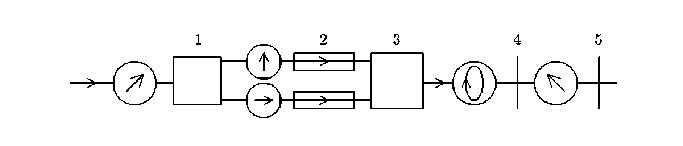
\includegraphics[scale=0.7]{Ris/ris_eps/ris2_07.eps}}}

\leftskip 0cm\centerline{\ris Рис. 2.7. Принципиальная схема
интерференционно-поляризационного рефрактометра.}

\noindent{\Small 1,3 --- поляризационные элементы, 2 --- кюветы со
сравниваемыми веществами, 4 --- пластинка << в четверть длины
волны>>, 5 --- анализатор.} \vskip 2mm На пути пучков помещается
кювета 2 со сравниваемыми веществами. Сведение пучков
осуществляется аналогичным поляризационным элементом 3. Суммарная
разность хода $\Delta_{\Sigma}$ после сведения пучков определяется
выражением:
$$\Delta_{\Sigma}=2\Delta+(n_2-n_1)l.\noq$$
Величина вносимой каждым поляризационным элементом разности хода
$\Delta$ является постоянной при достаточной температурной и
механической стабилизации поляризационных элементов и может быть
либо скомпенсирована, либо при достаточной временной когерентности
используемого излучения просто исключена из рассмотрения как
постоянная составляющая. Таким образом, можно считать, что при
данной длине кюветы $\Delta_{\Sigma}$ определяется только
величиной $n_2-n_1=\Delta n$, которой соответствует разность фаз
$\delta$:
$$\delta={2\pi\over\lambda}\Delta n\cdot l.\noq$$
Световые пучки равной интенсивности с разностью фаз $\delta$,
складываясь во втором поляризационном элементе, главное
направление которого ориентировано параллельно главному
направлению первого, дают эллиптически поляризованную волну,
причем большая ось эллипса либо параллельна, либо перпендикулярна
плоскости поляризации падающего света. Фазовая пластинка << в
четверть длины волны>>\ 4 с главными направлениями,
ориентированными параллельно осям эллипса, преобразуют
эллиптическое колебание в плоскополяризованное. Плоскость
поляризации выходящего из фазовой пластинки луча повернута
относительно первоначального плоскополяризованного луча на угол
$\psi={\delta\over2}$, связанный, согласно \eqn{48}, с разностью
показателей преломления $n_1$ и $n_2$ соотношением:
$$\Delta n={\lambda\over\pi l}\psi.\noq$$
Угол $\psi$ с помощью анализатора 5 может измеряться с точностью
до $0,001^{\circ}$, что при малой величине отношения
${\lambda\over l}$ обеспечивает высокую чувствительность
интерференционно-поляризационного метода.

Анализируя формулу \eqn{49} для сопоставления данных
интерференционно-поляризационного метода с аналогичными
параметрами интерферометра Рэлея, находим, что чувствительность
описываемого метода выше на четыре порядка, что позволяет с
миллиметровой кюветой достигнуть чувствительности измерения
вдесятеро более высокой, чем на метровой кювете обычного
лабораторного интерферометра. Высокая чувствительность
интерференционно-поляризационного метода нашла практическое
применение при изучении диффузионных процессов.

\zag{Дисперсия света}

\subzag{Элементарная классическая теория} \vskip 2mm Хорошо
известное наличие зависимости показателя преломления от частоты
падающего света представляет собой факт первостепенной важности.
Именно в этом вопросе феноменологическая электродинамика Максвелла
зашла в тупик. Явление дисперсии потребовало для своего объяснения
создания детализированной электронной теории. Во 2 главе была
установлена связь между показателем преломления (рефракцией) и
поляризуемостью атома или молекулы. Наличие дисперсии не нарушает
этой связи, но из факта зависимости показателя преломления от
длины волны следует, что сама поляризуемость является функцией
частоты света. Для понимания сущности явлений молекулярной оптики,
которые все, так или иначе, связаны с поляризуемостью, необходимо,
следовательно, нахождение вида зависимости поляризуемости от
частоты света, необходимо построение полной теории поляризуемости
с учетом дисперсионной зависимости.

Строгая молекулярная теория распространения света в веществе
изучает наложение вторичных световых волн, излучаемых молекулами,
возбужденными внешней электромагнитной световой волной. Эта теория
была разработана рядом авторов на основе представлений
кристаллооптики. Рассматривается плоская световая волна,
попадающая в изотропную среду. Под действием  поля волны $\vec E$
в молекулах среды индуцируются диполи, совершающие вынужденные
колебания с частотой, равной частоте световой волны. Эти диполи
являются источниками вторичных, на этот раз сферических световых
волн. Первое электрическое поле. действующее на данную молекулу
--- диполь $j$ слагается из внешнего поля $\vec E$ и полей
сферических волн, создаваемых остальными диполями:
$$\vec E'^{(j)}=\vec E+\sum_{l}E'^{(jl)}.\noq$$
В результате наложения первичной плоской волны и всех вторичных
волн, излучаемых всеми диполями среды, содержащей $N_1$ диполей в
единице объема, получается результирующая волна, которая, как
показывает расчет, является плоской. Внутри среды эта волна
распространяется в соответствии с законом преломления, вне ее ---
в соответствии с законом отражения.

В молекулярной теории, основывающейся на электронном рассмотрении,
волны, испускаемые диполями, распространяются от молекулы до
молекулы со скоростью света в вакууме $c$. Скоростью $c={c'\over
n}$ характеризуется лишь результирующая волна.

Весьма важным принципиальным результатом молекулярной теории
является отсутствие света по направлениям, отличным от направления
преломленного и отраженного лучей. Этот результат получается при
условии, что имеет место равномерное распределение вещества по
объему, и, следовательно, постоянное значение $N_1$. При этом
условии свет гасится по всем направлениям, кроме предписанных
законами волновой оптики, вследствие интерференции, так как
вторичные волны когерентны. Строгая теория приводит к соотношению:
$${n^2-1\over n^2+2}={4\pi\over3}N_1\alpha,$$
где $\alpha$ --- средняя поляризуемость молекул, причем постоянная
внутреннего поля ${4\pi\over3}$ получается, как непосредственное
следствие предполагаемой равномерности в распределении молекул.

Очевидно, что исследование дисперсии в рамках классической
волновой теории должно строиться на тех же основаниях. Поэтому мы
должны рассмотреть излучение и поглощение света элементарными
излучателями. Такими излучателями в электронной теории являются
электроны, совершающие гармонические колебания около положения
равновесия. Рассмотрим свободные колебания таких гармонических
осцилляторов. Они описываются уравнением движения:
$$m\ddot{\vec r}+k\vec r=0,\noq$$
где $m$ --- масса, $k$ --- упругая постоянная. Общее решение этого
уравнения имеет вид:
$$\vec r=\vec a\cos \omega_0t+\vec b\sin \omega_0t,\noq$$
где $$\omega_0=\sqrt{{k\over m}}.\noq$$ Колеблющийся электрон
имеет дипольный момент:
$$\vec p=e\vec r=e\vec a\cos \omega_0t+e\vec b\sin \omega_0t.\noq$$
Следовательно:
$$\ddot{\vec p}=-\omega_{0}^2\vec p.$$
В электродинамике доказывается, что поле нейтральной системы
зарядов на больших от нее расстояний совпадает в первом
приближении (при условии ${x_0\omega\over c}\ll 1$) с полем
диполя, момент которого равен моменту системы. Гармонический
осциллятор является источником сферических световых волн,
электрическая и магнитная напряженности которых выражаются в
волновой зоне (на расстояниях $R\gg x_0$) следующим образом:
$$\vec E={1\over c^2R^3}\left[\vec R\left[\vec R\ddot{\vec
p}\right]\right],\noq$$
$$\vec H=-{1\over c^2R^2}\left[\vec R\ddot{\vec
p\mathstrut}\right],\noq$$ откуда вектор Умова-Пойнтинга:
$$\vec S={c\over4\pi}[\vec E\vec H]={c\over4\pi}{1\over
c^{4}R^5}\vec R\left[\vec R\ddot{\vec p}\right]^2.\noq$$
Расположение векторов $\vec p$, $\vec E$, $\vec H$, $\vec R$ и
$\vec S$ показано на рис. 3.1. Интенсивность излучения по
некоторому направлению $\vec R$, составляющему угол $\vartheta$ с
направлением колебания осциллятора, выражается величиной:
$$|\vec S|={1\over 4\pi c^3R^2}\left(\ddot{\vec
p}\right)^2\sin^2\vartheta.\noq$$

\vskip 3mm
\centerline{\hbox{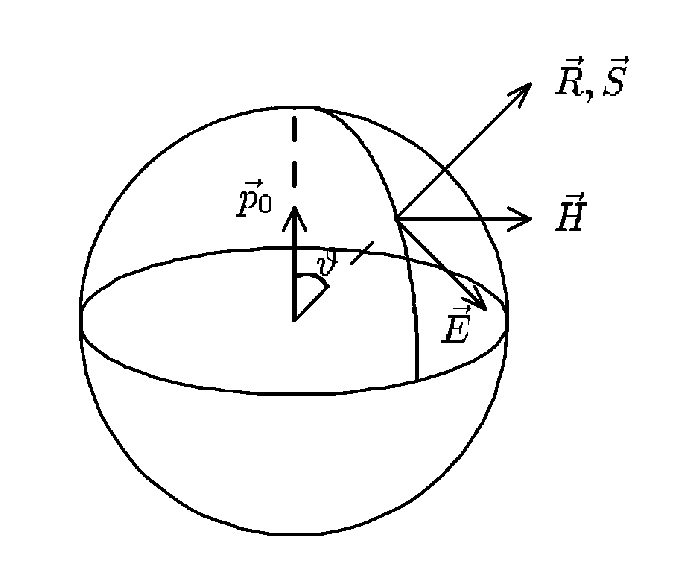
\includegraphics[scale=0.7]{Ris/ris_eps/ris3_01.eps}}}

\leftskip 0cm\centerline{\ris Рис. 3.1. Излучение колеблющегося
диполя.} \vskip 2mm Подставляя в \eqn{9} значение $\vec
p=-\omega^2_0\ddot{\vec p}$, находим:
$$|\vec S|={1\over4\pi c^3R^2}\omega^4_0\vec p^2\sin^2\vartheta.\eqno
(3.9a)$$ Общая энергия, излучаемая осциллятором в единицу времени,
есть интеграл от $|\vec S|$ по сферической поверхности:
$${dW\over dt}=\int\int|\vec S|R^2\sin\vartheta d\vartheta
d\varphi={2\over3}{\omega_0^4\over c^3}\overline{p^2}.\noq$$ Здесь
$\overline{p^2}$ --- среднее значение $p^2$ за данный промежуток
времени. В силу соотношений \eqn{5-7}, имеем:
$$\vec E={\omega_0^2\over c^2R^3}\left[\vec R\left[\vec p\vec
R\right]\right]=\vec E_1\cos \omega_0t+\vec E_2\sin
\omega_0t,\noq$$
$$\vec H={\omega_0^2\over c^2R^3}\left[\vec p\vec
R\right]=\vec H_1\cos \omega_0t+\vec H_2\sin \omega_0t.\noq$$
Иными словами, сферическая волна, испускаемая гармоническим
осциллятором, есть монохроматическая волна с частотой $\omega_0$,
той же самой, с которой колеблется осциллятор. Однако, в силу
\eqn{10}, осциллятор не может колебаться по закону \eqn{2}, ибо он
не непрерывно отдает свою энергию в виде излучения и его энергия
колебаний, в отсутствие внешней силы, их поддерживающей,
непрерывно уменьшается, --- колебания затухают.

Для того, чтобы удовлетворить закону сохранения энергии, мы должны
ввести в уравнение движения добавочную силу --- такую, чтобы ее
наличие определяло потерю энергии в соответствии с \eqn{10}.
Напишем:
$$m\ddot{\vec r}+k\vec r=\vec K,\noq$$
и после умножения на $\dot{\vec r}$:
$${d\over dt}\left({m\over2}\ddot{\vec{r^2}}+{k\over2}\vec{r^2}\right)=\vec K\dot{\vec r}.$$
Здесь слева стоит изменение энергии ${dW\over dt}$ --- ее
уменьшение. Следовательно:
$$\vec K\overline{\dot{\vec r}}=-{2\omega_0^4\over3c^3}\overline{p^2}=
-{2e^2\over3c^3}\overline{\ddot{\vec{r^2}}},$$ и, так как
$${d\over dt}\left(\dot{\vec r}\ddot{\vec
r}\right)\equiv\ddot{\vec r}+\dot{\vec r}\tridot{\vec r},$$ имеем
среднее значение $\vec K\dot{\vec r}$ в интервале от $t=0$ до
$t=T$:
$$\overline{\vec K\dot{\vec
r}}={2e^2\over3c^2}\overline{\tridot{\vec r}\dot{\vec r}}.\noq$$
Мы удовлетворим нашим условиям в среднем, положив
$$\vec K={2e^2\over3c^3}\tridot{\vec r},\noq$$
и для почти периодических движений:
$$\vec K=-{2e^2\omega_0^2\over3c^3}\dot{vec r}.\noq$$
Уравнение движения принимает вид:
$$m\ddot{\vec r}+m\gamma\dot{\vec r}+k\vec r=0,\noq$$
где
$$\gamma={2e^2\over3c^3m}.$$
Благодаря наличию члена $m\gamma\dot{\vec r}$, характеризующего
силу трения, амплитуда колебаний будет затухать. Получаем решение
\eqn{17}, аналогичное \eqn{3}, причем:
$$\vec a=\vec a_0e^{-\gamma/2t},\hskip 4mm \vec b=\vec
b_0e^{-\gamma/2t}.$$ Итак, решение \eqn{17} имеет вид:
$$\vec r=e^{-\gamma/2t}(\vec a_0\cos \omega_0t+\vec b_0\sin \omega_0t).\noq$$
Это решение, как легко видеть, удовлетворяет уравнению \eqn{13}
при малом затухании, т.е. в случае $\gamma\ll \omega_0$. Нетрудно
убедиться, что решение \eqn{18} соответствует потере энергии
\eqn{10}. Определив $\vec r$, как $\vec r=\vec Ae^{i\omega_0t}$,
где $\vec A$ --- комплексный вектор, напишем:
$$\vec p=e\vec r=\vec p_0e^{-\gamma/2t}e^{i\omega_0t},\noq$$
и, согласно \eqn{11}, \eqn{12},
\begin{plain}$$\eqalign{\vec E=&\vec E_0e^{-\gamma/2t}e^{i\omega_0t},\cr
\vec H=&\vec H_0e^{-\gamma/2t}e^{i\omega_0t}, }\noq$$\end{plain} где $p_0$,
$E_0$, $H_0$ --- комплексные амплитуды. Волна \eqn{20} уже не
является монохроматической, но характеризуется некоторым
распределением интенсивностей по частотам $\omega$. Чтобы найти
это распределение, разложим \eqn{20} в интеграл Фурье: \vskip -2mm
\begin{plain}$$\eqalign{
&\vec E={1\over2}\int\limits_{-\infty}^{+\infty}\vec
E(\omega)e^{i\omega t}d\omega, \cr &{\rm где} \cr &\vec
E(\omega)={1\over2\pi}\vec
E_0\int\limits_0^{+\infty}e^{i(\omega_0-\omega)t}e^{-\gamma/2t}dt
.} \noq$$\end{plain} Имеем: \vskip -2mm
$$\vec E(\omega)={1\over2\pi}\vec E_0{1\over i(\omega_0-\omega)-\gamma/2},$$
и распределение интенсивностей: \vskip -2mm
$$I(\omega)\cong|\vec E(\omega)|^2=I_0{\gamma\over2\pi}{1\over
(\omega_0-\omega)^2-(\gamma/2)^2},\noq$$ где $I_0$ ---
интегральная интенсивность, равная
$\int\limits_{-\infty}^{+\infty}I(\omega)d\omega$.

Вид кривой $I(\omega)$ представлен на рис. 3.2. Кривая имеет
максимум при $\omega=\omega_0$ (точнее, максимум слегка сдвинут
относительно $\omega_0$, но сдвигом можно пренебречь, так как
${\gamma\over \omega_0}\ll 1$). Мы можем охарактеризовать ширину
линии (полосы) излучения интервалом значений $\omega$, в котором
$I(\omega)$ имеет величину больше половины максимальной
$I(\omega_0)$, равной: \vskip -2mm
$$I(\omega)=I_0{2\over\pi\gamma}.$$

\vskip 3mm
\centerline{\hbox{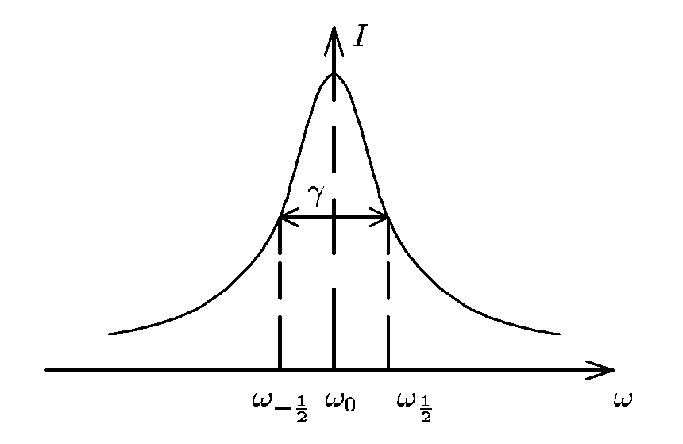
\includegraphics[scale=0.7]{Ris/ris_eps/ris3_02.eps}}}

\vskip -2mm
\leftskip 0cm\centerline{\ris Рис. 3.2. Контур спектральной
линии.} \vskip 2mm Ищем значения $\omega$, при которых
$$I(\omega_{1\over2})={1\over2}I(\omega_0)=I_0{1\over\pi\gamma},$$
имеем:
$$\omega_{1\over2}=\omega_0\pm{\gamma\over2}.$$
Следовательно, полуширина спектральной линии, излучаемой
затухающим осциллятором, дается значением:
$$\Delta \omega=\gamma.\noq$$

Укажем, что затухание вследствие излучения и соответствующее
расширение спектральной линии обычно малы по сравнению с
затуханием и расширением, вызванными другими причинами:
соударениями между излучающими частицами, влиянием электрического
поля, явлением Доплера и т.д. Во всех этих случаях по-прежнему
применимо уравнение \eqn{17}.

Перейдем теперь к нашей непосредственной задаче, к рассмотрению
явления дисперсии. Рассмотрим электрон --- гармонический
осциллятор, находящийся под действием внешней световой волны.
Пренебрегая затуханием, мы напишем уравнение движения в виде:
$$m\ddot x+kx=eE_x,\noq$$
где $E_x$ --- напряженность поля световой волны, действующей на
электрон с зарядом $e$. Переходя сразу к дипольному моменту,
получим:
$$\ddot{\vec p}+\omega_0^2\vec p={e^2\over m}\vec E.\noq$$
Но поле $\vec E$ --- поле световой волны периодически зависит от
времени с частотой падающего света:
$$\vec E=\vec E_0e^{i\omega t}.\noq$$
Следовательно, уравнение \eqn{25} есть уравнение вынужденных
колебаний. Ищем его решение в виде:
$$\vec p=\vec p_0e^{i\omega t}.\noq$$
Подставляя в \eqn{25}, имеем:
$$\vec p(\omega_0^2-\omega^2)={e^2\over m}\vec E,$$
откуда:
$$\vec p={e^2\over m}{1\over \omega_0^2-\omega^2}\vec E=\alpha\vec E.\noq$$
Т.е. поляризуемость гармонического осциллятора зависит от частоты
внешнего поля по дисперсионному закону:
$$\alpha={e^2\over m}{1\over \omega_0^2-\omega^2}.\noq$$
В статическом поле $\omega=0$ и
$$\alpha={e^2\over m\omega_0^2}={e^2\over k}.\noq$$
Здесь мы говорим о некотором скалярном осцилляторе, колеблющемся в
том же направлении, что и $\vec E$, и, соответственно, о скалярной
поляризуемости $\alpha$. Очевидно, что подобное рассмотрение
применимо и к поведению среднего дипольного момента,
индуцированного полем.

В этих рассуждениях мы пренебрегли влиянием магнитного поля. В
теории дисперсии оно мало существенно. Но им нельзя пренебрегать в
тех случаях, когда мы рассматриваем действие сильного внешнего
магнитного поля. В этом случае вместо уравнения \eqn{24} напишем:
$$m\ddot x+kx=eE_x+{e\over c}\left[\dot{\vec r}\vec
H\right]_x.\eqno (3.24a)$$ Магнитное поле создает действующую на
электрон силу Лорентца. Здесь $\vec r=\vec r(x,y,z)$. При
одинаковых порядках величины $E$ и $H$ (поле световой волны),
магнитная сила много меньше электрической, ибо:
$${|\dot{\vec r}|\over c}\ll 1.$$
Согласно \eqn{29}, поляризуемость становится бесконечно большой,
когда частота внешнего поля совпадает с собственной частотой
осциллятора --- с той частотой, которую он сам излучает.

По основному закону спектроскопии --- закону Кирхгоффа -- эта
частота есть, тем самым, частота поглощения осциллятора.

Значение $\alpha\rightarrow\infty$ парадоксально и получилось
потому, что мы пренебрегли затуханием. Учтем это обстоятельство:
$$\ddot p+\gamma\dot p+\omega_0^2p={e\over m}E_0e^{i\omega t}.\noq$$
По-прежнему ищем решение в виде \eqn{27}. Получаем:
$$p=\alpha E={e^2\over m}{1\over \omega_0^2-\omega^2+i\omega\gamma}E.\noq$$
Мы получили комплексное выражение для поляризуемости. Для того,
чтобы раскрыть его смысл, вернемся к формуле Лоренц-Лоренца
\eqn{18}. Подставив в нее полученное выражение для $\alpha$,
имеем:
$${\tilde n^2-1\over\tilde n^2+2}={4\pi\over3}N_1={4\pi\over3}N_1
{e^2\over m}{1\over \omega_0^2-\omega^2+i\omega\gamma},\noq$$ где
$\tilde n$ --- комплексный показатель преломления. Для газов:
$$\tilde n=1+2\pi N_1{e^2\over m}{1\over
\omega_0^2-\omega^2+i\omega\gamma}.\noq$$ Представим комплексный
показатель в виде:
$$\tilde n=n-i\chi.\noq$$
Результирующая плоская волна в среде --- преломленная волна ---
может быть представлена выражением:
$$E=E_0e^{i\omega\left(t-{\tilde n R\over
c}\right)}=E_0e^{-{\chi \omega R\over
c}}e^{i\omega\left(t-{nR\over c}\right)}.\noq$$ Таким образом,
мнимый член в $\tilde n$ характеризует затухание проходящей волны
по мере прохождения ею пути $R$. Коэффициент $\chi$ называется
коэффициентом экстинкции и выражает поглощение света в веществе.
Действительно, согласно уравнению \eqn{36}, интенсивность
проходящего света должна ослабляться в поглощающей среде по
закону:
\begin{plain}
$$\eqalign{I=&I_0e^{-kR},\cr
k=&2{\chi \omega\over c}.}\noq$$ Вычислим $n$ и $\chi$. Для газов
получаем, согласно \eqn{34}:
$$n-i\chi=1+2\pi N_1{e^2\over m}\left\{{\omega_0^2-\omega^2\over
(\omega_0^2-\omega^2)^2+\gamma^2\omega^2}-i{\gamma
\omega\over(\omega_0^2-\omega^2)^2+\gamma^2\omega^2}\right\},$$
откуда
$$\eqalign{n=&1+2\pi N_1{e^2\over m}{\omega_0^2-\omega^2\over
(\omega_0^2-\omega^2)^2+\gamma^2\omega^2},\cr \chi=&2\pi
N_1{e^2\over m}{\gamma
\omega\over(\omega_0^2-\omega^2)^2+\gamma^2\omega^2}.}$$ 
\end{plain}
Ход
$n(\omega)$ показан на рис. 3.3. Мы видим, что ход $\chi$ связан с
видом линии (полосы) поглощения, полуширина которой $\Delta
\omega=\gamma$.

В области, удаленной от собственной частоты поглощения можно
пренебречь значением $\gamma^2\omega^2$ в знаменателе по сравнению
с $(\omega_0^2-\omega^2)$, и, на равных основаниях, пренебречь
мнимым членом в выражении поляризуемости. Здесь справедливо
выражение для поляризуемости \eqn{29}:
$$\alpha={e^2\over m}{1\over \omega_0^2-\omega^2}.$$

\vskip 3mm
\centerline{\hbox{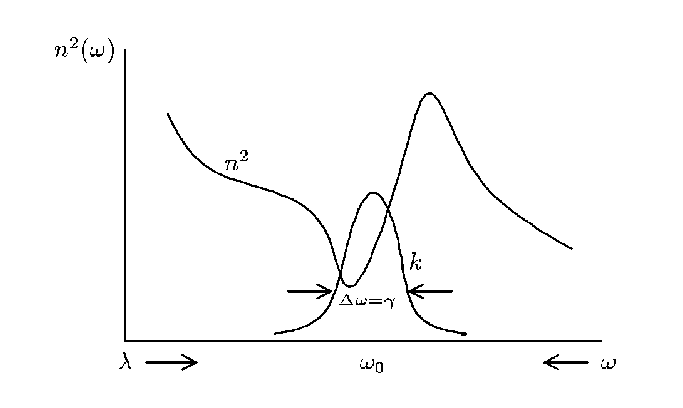
\includegraphics[scale=0.7]{Ris/ris_eps/ris3_03.eps}}}

\leftskip 0cm\centerline{\ris Рис. 3.3. Кривая дисперсии.} \vskip
2mm Однако реальная система --- атом, молекула, обладает не одной,
а целым набором собственных частот $\omega_0$, наблюдаемых в
спектре испускания или поглощения. С точки зрения классической
электронной теории, мы должны с каждой частотой сопоставить
некоторый гармонический осциллятор с зарядом и массой $e_i$,
$m_i$. Обозначим:
$${e_i^2\over m_i}=f_i{e^2\over m},$$
где $e$ и $m$ --- заряд и масса электрона. Поляризуемость всей
системы представится выражением:
$$\alpha={e^2\over m}\sum_{i}{f_i\over \omega_i^2-\omega^2}={b\over3},\noq$$
причем сумма всех $f_i$ должна равняться полному числу
осцилляторов-электронов в рассматриваемой системе:
$$\sum_{i}f_i=Z.\noq$$
Безразмерные величины $f_i$ называются силами осцилляторов, $f_i$
могут, конечно, быть нецелыми числами и, в частности, возможны
значения $f_i\ll 1$.

Очевидно, что $f_i$ характеризуют интенсивность линий (полос)
испускания и поглощения системы. В самом деле, при учете
затухания, согласно \eqn{34}:
$$\tilde n=1+2\pi N_1{e^2\over m}\sum_{i}{f_i\over
\omega_i^2-\omega^2+i\gamma_i \omega},$$ и для каждой отдельной
полосы получаем:
$$\chi_{\omega=\omega_i}=2\pi N_1{e^2\over m}{f_i\over\gamma_i\omega_i}.$$
Коэффициент экстинкции $\chi_i$ и коэффициент поглощения $k_i$
пропорциональны $f_i$.

Схематически ход дисперсии показателя преломления в случае
нескольких полос поглощения представлен на рис. 3.4.

\vskip 3mm
\centerline{\hbox{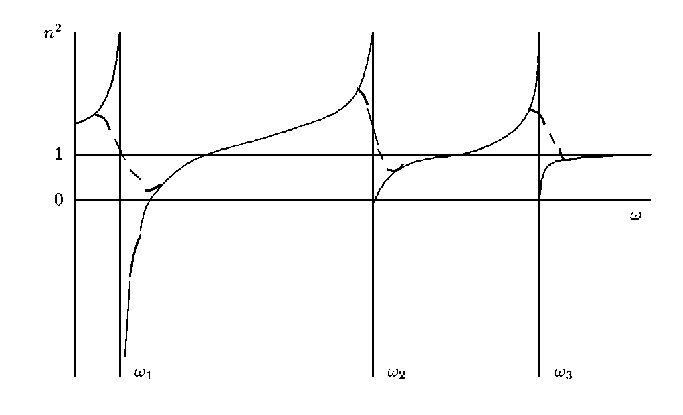
\includegraphics[scale=0.7]{Ris/ris_eps/ris3_04.eps}}}

\leftskip 0cm\centerline{\ris Рис. 3.4. Кривая дисперсии при
наличии нескольких полос поглощения.} \vskip 2mm Так как измерения
показателя преломления (рефракции) обычно производятся в
прозрачной, т.е. достаточно удаленной от собственных полос
поглощения спектральной области, можно пользоваться формулой, в
которой не учитывается затухание. Окончательно получаем:
$${n^2-1\over n^2+2}={4\pi\over3}N_1\sum_{i}{f_i\over
\omega_i^2-\omega^2},\noq$$
$$R={n^2-1\over n^2+2}{M\over\rho}={4\pi\over3}N_A{e^2\over
m}\sum_{i}{f_i\over \omega_i^2-\omega^2}.\eqno (3.41a)$$

\subzag{Квантовомеханическая теория дисперсии.} \vskip 2mm Выше мы
ограничились краткими сведениями по классической теории дисперсии.
Наиболее важным и общим результатом классической электронной
теории дисперсии является установление тесной связи между
дисперсией и поглощением света. Недостатком классической теории
является формальный характер введения сил осцилляторов $f_i$,
характеризующих степень участия электрона в данном колебании.

Обычный метод рассмотрения взаимодействия вещества со светом
состоит в квантовании частиц вещества, но сохранении для
электромагнитного поля света классических выражений. Это возможно
на основании принципа соответствия. При квантовании атома или
молекулы мы должны отказаться от классической модели
гармонического осциллятора. Однако, в квантовомеханической теории
излучения, исходящей из комбинационного принципа, связывающего
частоту испускаемой или поглощаемой световой волны с разностью
энергий комбинирующих уровней:
$$\hbar \omega_{mn}=E_m-E_n.\noq$$
Интенсивность соответствующей спектральной линии испускания или
поглощения выражается через вероятность перехода $m\leftrightarrow
n$. Большей частью в оптике приходится встречаться с
квантовомеханическими переходами дипольного характера. Их
вероятности определяются матричными элементами электрического
дипольного момента:
$$\vec p_{mn}=\int\psi_m^*\vec p\psi_nd\tau=e\int\psi_m^*\vec
r\psi_nd\tau,\noq$$ и интенсивность, точнее --- величина обще
энергии, излучаемой в единицу времени при переходе
$m\leftrightarrow n$ дается уравнением:
$${dW\over dt}={4\over3}{\omega^4_{mn}\over c^3}|\vec p_{mn}|^2.\noq$$

Решая волновое уравнение для гармонического осциллятора, мы
находим собственные функции $\psi_n$ и, следовательно, приобретаем
возможность вычисления матричных элементов \eqn{43}. Расчет
показывает, что матричный элемент отличен от нуля только для таких
переходов, при которых квантовое число $n$ меняется на $\pm 1$.
Тем самым:
$$\omega_{mn}=\omega_{n+1,n}={1\over\hbar}(E_{n+1}-E_n)={\hbar \omega\over\hbar}
\left(n+{3\over2}-n-{1\over2}\right)=\omega,\noq$$ т.е. частота,
излучаемая (или поглощаемая) гармоническим осциллятором, согласно
квантовой механике, совпадает с его классической собственной
частотой колебаний. Квантовомеханическое поведение гармонического
осциллятора не отличается в этом смысле от классического.
Величина, которая в квантовой механике совпадает с классической
собственной частотой колебаний осциллятора, не зависит от
амплитуды его колебаний. << Квантуется>> именно амплитуда.
Указанным свойством совпадения результатов квантовомеханического и
классического рассмотрения процессов испускания и поглощения света
обладает только гармонический осциллятор. Его частота не
квантуется.

Что касается выражений \eqn{43} и \eqn{44}, характеризующих
интенсивность излучения, интенсивность спектральной линии, то эти
соотношения ограничены случаем излучения электрического диполя.
Именно электрическое дипольное излучение и поглощение обладает
наибольшей интенсивностью и именно с ним приходится иметь дело в
большинстве оптических явлений. Легко видеть, что формула \eqn{44}
аналогична классическому выражению \eqn{10} для общей энергии,
излучаемой гармонически-колеблющимся электрическим диполем. Эти
формулы совпадут, если принять:
\begin{plain}$$\eqalign{
&\omega_0=\omega_{mn},\cr &(\overline{p^2})_{\rm классич.}=2|\vec
p_{mn}|^2. }\noq$$ 
\end{plain} Множитель 2 возникает вследствие возможности
двух независимых направлений поляризации излучения
квантовомеханической системы, перпендикулярных к лучу. Таким
образом, имеется прямое соответствие между излучением, относящимся
к переходу $m\rightarrow n$ и излучением некоторого осциллятора,
характеризуемого условиями \eqn{46}.

Таким образом, при характеристике оптических свойств атома или
молекулы (ограничиваясь рассмотрением дипольных моментов) приходим
к выводу о соответствии классических и квантовомеханических
выражений.

Классическому осциллятору с частотой $\omega_0$ и силой
осциллятора $f$, определяющей интенсивность линии в спектре,
соответствует матрица частот:
$$\omega_{mn}={1\over\hbar}(E_m-E_n);$$
$$\left|\matrix{
0&\omega_{12}&\cdots&\omega_{1n}&\cdots\cr
\omega_{21}&0&\cdots&\omega_{2n}&\cdots\cr
\cdots&\cdots&\cdots&\cdots&\cdots\cr
\omega_{m1}&\omega_{m2}&\cdots&\omega_{mn}&\cdots\cr
\cdots&\cdots&\cdots&\cdots&\cdots\cr }\right|,$$ и матрица <<
амплитуд>>\ электрического момента:
$$\left|\matrix{
p_{11}&p_{12}&\cdots&p_{1n}&\cdots\cr
p_{21}&p_{22}&\cdots&\omega_{2n}&\cdots\cr
\cdots&\cdots&\cdots&\cdots&\cdots\cr
p_{m1}&p_{m2}&\cdots&p_{mn}&\cdots\cr
\cdots&\cdots&\cdots&\cdots&\cdots\cr }\right|.$$ Диагональные
элементы матрицы $p_{mn}(t)$ не зависят от времени, так как, по
определению, $\omega_{nn}=0$. При этом интенсивности (>> силы
осцилляторов<<) выражаются через элементы матрицы \eqn{48}
следующим образом:
$$f_{nk}={2m|p_{nk}|^2\omega_{kn}\over3e^2\hbar}.\noq$$
Различие в точках зрения проявляется в частном случае
одноэлектронной системы (орбитальная модель атома водорода) в том,
что согласно классической теории, в такой системе имеется один
электрон с $f=1$ и определенной частотой $\omega_0$ и,
следовательно, поляризуемость может быть выражена одночленной
дисперсионной формулой, а согласно квантовой механике, уже в такой
системе мы имеем целый набор осцилляторов, характеризуемый
матрицами \eqn{47} и \eqn{48}, и, следовательно, дисперсионная
формула должна, по аналогии с классической формулой \eqn{39},
выражаться суммой. В общем случае:
$$\alpha={e^2\over m}\sum_n\sum_k \omega_n{f_{nk}\over
\omega^2_{nk}-\omega^2}.\noq$$ Здесь $\omega_n$ --- вероятность
того, что система находится в состоянии с энергией $E_n$. Можем
принять по Больцману:
$$\omega_n=e^{-{E_n\over kT}}.$$
Так как энергия возбуждения электронов, как правило, значительно
больше $kT$, мы можем практически отвлечься от
электронно-возбужденных состояний и, отсчитывая энергию от
основного уровня с $n=0$, положить $\omega_0=1$. Следовательно:
$$\alpha={e^2\over m}\sum_{k}{f_{0k}\over \omega^2_{0k}-\omega^2}.\eqno
(3.50a)$$ Существенно новым результатом квантовомеханического
рассмотрения по сравнению с классической теорией является
объяснение отрицательной дисперсии. В классической теории все
величины $f_i>0$. В квантовой теории такого ограничения нет. Если
мы имеем дело с электронно-возбужденным состоянием с энергией
$E_n$, то некоторые из $f_{nk}$ могут быть отрицательны, а именно
те, для которых $\omega_{kn}<0 (E_k<E_n)$. При этом ход дисперсии
может стать обратным обычному (рис. 3.5). Явление отрицательной
дисперсии действительно удается наблюдать при определенных
условиях.

\vskip 3mm
\centerline{\hbox{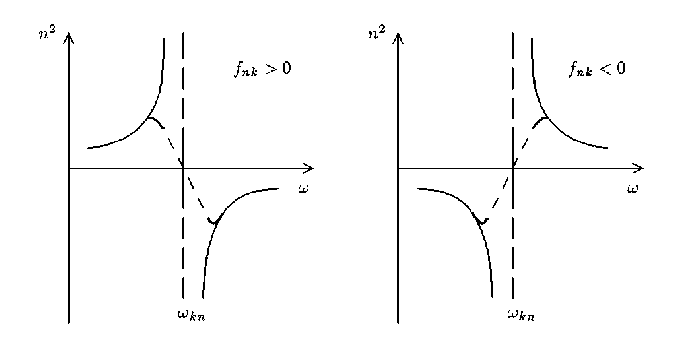
\includegraphics[scale=0.7]{Ris/ris_eps/ris3_05.eps}}}

\leftskip 0cm\centerline{\ris Рис. 3.5. Положительная и
отрицательная дисперсия.} \vskip 2mm Теоретическое вычисление
$f_{nk}$ требует знания волновых функций $\psi_n,\ \psi_k$
системы. В настоящее время такие расчеты пока невозможны. Величины
$f_{nk}$ определяются из опыта, который может с полным правом быть
истолкован при помощи классических соображений. Существует два
замечательных экспериментальных метода исследования дисперсионных
явлений, дающих возможность с высокой точностью определить ход
дисперсии и силы осцилляторов. Это метод крюков Д. С.
Рождественского и дифракционный метод И. В. Обреимова. Описание
данных методов можно найти в курсе << Молекулярная оптика>>\ М.
В. Волькенштейна и в сборнике Д. С. Рождественского << Природа
света>>.

Как показывает квантовая механика, величины $f_{nk}$ удовлетворяют
условию суммы, которое может рассматриваться, как аналогичное
\eqn{40}. Квантовая механика показывает, что для каждого
электрона, находящегося в состоянии, характеризуемом квантовым
числом $n$, имеет место условие:
$$\sum_{k}f_{nk}=1;\noq$$
$$\sum\limits_{\rm по\ всем\
электронам}\left(\sum_{k}f_{nk}\right)=Z.\eqno (3.51a)$$ Здесь
суммирование распространяется по всем электронам, участвующим в
процессе.

Таким образом, сопоставление данных классической и
квантовомеханической теории дисперсии показывает, что решая
проблемы, связанные с электрическим дипольным излучением и
поглощением свет, мы вправе пользоваться простой классической
моделью гармонического осциллятора. Численные значения
фигурирующих в наших формулах величин --- частот и сил
осцилляторов --- могут быть найдены теоретически только в
квантовой механике, поскольку атом или молекула являются
микрообъектами, недоступными рассмотрению в рамках классической
теории. Однако ввиду практической невозможности решения волнового
уравнения для многоэлектронной системы, приходится пользоваться
опытными значениями частот и интенсивностей, причем можно
трактовать их классически. Следовательно, теория явлений, так или
иначе связанных с излучением и поглощением --- с дисперсией света
в веществе, может разрабатываться в настоящее время как
классическая полуэмпирическая теория, в основу которой положена
модель гармонического осциллятора.

\subzag{Дисперсия и рефракция.} \vskip 2mm Рассмотрим опытные
данные, характеризующие ход дисперсии в некоторых чистых
веществах. Наблюдаемый ход дисперсии принято выражать
эмпирическими формулами, в которых обычно удается ограничиться
небольшим числом членов. Одночленной формулой можно пользоваться в
тех случаях, когда все полосы поглощения, кроме ближайшей,
обладающей частотой $\omega_0$, либо лежат в далекой области
$\omega_i\gg \omega$, либо обладают малыми силами осцилляторов
$f_i$:
$$n\cong1+2N_1{e^2\over m}{f\over \omega_0^2-\omega^2}.\noq$$
Экстраполируя значение рефракции к бесконечно большим длинам волн,
находим среднюю статическую поляризуемость $\alpha^{\circ}$. Имеем
для оптической поляризуемости формулу:
$$\alpha_{\rm опт.}={e^2\over m}\sum_{i}{f_i\over \omega_i^2-\omega^2},\noq$$
и, положив $\omega=0$, получаем среднюю статическую
поляризуемость:
$$\alpha^{\circ}={e^2\over m}\sum_{i}{f_i\over \omega_i^2}.\noq$$
Величины $\alpha_{\rm опт.}$ и $\alpha^{\circ}$ тем ближе друг к
другу, чем дальше лежит полоса поглощения $\omega_i$ от той
области спектра, в которой мы проводим измерения. Рассмотрим
пример. Допустим, что длина волны падающего света
$\lambda=5000\angst$, а собственная полоса поглощения лежит при
$\lambda_0=1000\angst$. Тогда величина
$${1\over
\omega_0^2-\omega^2}={1\over4\pi^2c^2}{\lambda_0^2\lambda^2\over\lambda^2-\lambda_0^2}=
{1\over4\pi^2c^2}\cdot1,04\cdot10^{6}\angst^2$$ всего на 4\%
отличается от величины
$${1\over
\omega_0^2}={1\over4\pi^2c^2}\lambda^2_0={1\over4\pi^2c^2}\cdot1,00\cdot10^6\angst^2.$$
Напротив, если полоса поглощения лежит в области, близкой к
области измерения, различие между оптической и статической
поляризуемостью значительно. Допустим, что по-прежнему
$\lambda=5000\angst$, но $\lambda_0=4000\angst$. Имеем:
$${1\over{\omega_0^2-\omega^2}}={1\over4\pi^2c^2}\cdot44,4\cdot10^6\angst^2,$$
$${1\over \omega_0^2}={1\over4\pi^2c^2}\cdot16\cdot10^6\angst^2.$$
Расхождение в этом случае приближается к 300\%.

Отсюда следует, что для веществ, обладающих только полосами
поглощения, расположенными в далекой ультрафиолетовой области
спектра, практически допустимо отождествление статической
поляризуемости с оптической в видимом спектре. Здесь
следовательно:
$$n^2\cong\varepsilon.\noq$$
Такого рода спектрами обладают, например, предельные углеводороды.
Заметные расхождения нет только между $n^2$ и $\varepsilon$, но и
$n_{\infty}^2$ и $\varepsilon$ у $\rm CO_2$, $\rm CO$, $\rm CH_4$,
$\rm C_2H_4$, а также тот факт, что в действительности почти
всегда $n^2_{\infty}<\varepsilon$ связаны с наличием атомной
рефракции.

Для веществ, обладающих полосами поглощения в близкой
ультрафиолетовой и видимой области, отождествление статической и
оптической поляризуемости невозможно. В этих случаях мы
непосредственно сталкиваемся с аномальной дисперсией. Приближение
к собственной полосе поглощения в области аномальной дисперсии
резко повышает поляризуемость (показатель преломления) вещества.

Выше указывалось, что чередование двойных и единичных $C-C$ связей
приводит к нарушению аддитивности рефракции, к экзальтации.
Очевидно, что само значение экзальтации должно зависеть от длины
волны света. Поэтому важно выяснить, определяется ли аномальное
повышение рефракции действительным следствием специфической
структуры молекулы, или мы просто попадаем, измеряя рефракцию, в
область длин волн, близкую к собственным полосам поглощения --- в
область аномальной дисперсии.

Рассмотрим случай паранитроанилина:

\vskip 3mm
\centerline{\hbox{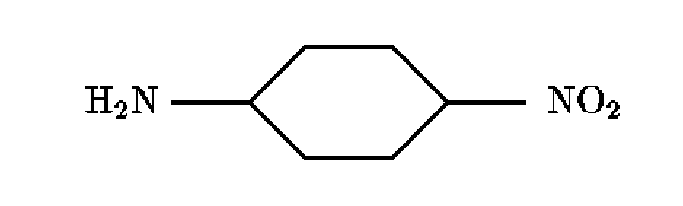
\includegraphics[scale=0.7]{Ris/ris_eps/ris3_05a.eps}}}

\leftskip 0cm Измерение рефракции при $\lambda=4358\angst$ (синяя
линия ртутного спектра) дает весьма высокое значение экзальтации,
равное $14,85\rm\ см^{3}$. Однако это значение быстро уменьшается
с увеличением длины волны света. Имеем:
\begin{plain}$$\eqalign{
\Delta R_{4358}=&14,85\ {\rm см^{3}},\cr \Delta R_{5460}=&7,01\
{\rm см^{3}},\cr \Delta R_{5790}=&6,40\ {\rm см^{3}},\cr \Delta
R_{6707}=&5,23\ {\rm см^{3}},\cr \Delta R_{\infty}=&2,70\ {\rm
см^{3}} }$$ \end{plain}
очевидно, что освещая п-нитроанилин светом с
$\lambda=4358\angst$, мы попадаем в область, близкую к аномальной
дисперсии. В самом деле, п-нитроанилин имеет полосу поглощения при
$\lambda=3200-4050\angst$ (в зависимости от растворителя).
Истинный физический смысл имеет экзальтация статическая ---
экстраполированная к нулевой частоте световой волны. Эти
обстоятельства всегда следует иметь в виду при оптической
характеристике вещества.

Из изложенного выше очевидно, что подлинное физическое содержание
аддитивности или неаддитивности рефракции может быть установлено
лишь на основе спектроскопических данных. Поляризуемость молекулы
есть специфическое проявление ее спектра --- она непосредственно
определяется совокупностью энергетических уровней и вероятностями
переходов между ними.

Все органические соединения обладают полосами поглощения, лежащими
в далекой ультрафиолетовой шумановской области спектра. Эта
область простирается от 1800 \angst\ в сторону меньших длин волн.
Если других полс поглощения нет (например, насыщенные
углеводороды), то рефракция аддитивна. Неаддитивные соединения
--- это соединения, содержащие так называемые хромофорные группы:
сопряженные связи, ароматические кольца, группы $\rm >C=O$, $\rm
-C\equiv C-$, $\rm -N\equiv N-$, $-NO_2$ и т.д.

Наличие этих групп определяет цветность органических соединений
--- сдвиг полос поглощения в длинноволновую область. Тем самым,
хромофорные группы определяют наличие экзальтации рефракций у
соответствующих соединений.

В практическом и принципиальном отношении весьма важен вопрос о
влиянии межмолекулярного взаимодействия на рефракцию и дисперсию
вещества. Во-первых, существенно прямое влияние межмолекулярных
сил на спектр и, тем самым, на поляризуемость. Во-вторых, не
следует забывать, что в выражении для рефракции фигурирует средняя
поляризуемость, получаемая из усреднения по всем равновероятным
ориентациям молекулярного хаоса. Однако взаимная ориентация
молекул, вызванная межмолекулярными силами, может привести к
изменению статистики и, следовательно, к изменению значения
поляризуемости (здесь нельзя уже использовать поляризуемость,
получаемую при усреднении по всем равновероятным ориентациям).

\subzag{Аналитические применения дисперсионной формулы.} \vskip 2mm
Перейдем теперь к некоторым аналитическим применениям
дисперсионной формулы. Дисперсия является важным аналитическим
признаком для вещества. Можно характеризовать вещество величиной
молекулярной дисперсии --- разности молекулярных рефракций для
определенных длин волн:
$$D_{12}=R_{\lambda_1}-R_{\lambda_2}={M\over\rho}\left\{
{n_1^2-1\over n_1^2+2}-{n_2^2-1\over n_2^2+2}\right\}.\noq$$
Величины типа также должны обладать аддитивностью в тех случаях,
когда имеет место аддитивность рефракций. Имеем, следовательно:
$$D_{12}=\sum_i(D_{12})_i.\noq$$
В ряде случаев сопоставление наряду с молекулярными рефракциями
также и молекулярных дисперсий позволяет повысить точность
структурного анализа вещества.

Наличие дисперсионной зависимости позволяет, исходя из
аддитивности молекулярных рефракций, анализировать
многокомпонентные смеси. Рассмотрим случай трехкомпонентной смеси.
Имеем уравнения:
\begin{plain}
$$\eqalign{
&c_1+c_2+c_3=1,\cr &R_1c_1+R_2c_2+R_3c_3=R,\cr
&R'_1c_1+R'_2c_2+R'_3c_3=R', }\noq$$ 
\end{plain}
где $c_1$, $c_2$, $c_3$ ---
молярные доли трех компонент. Здесь величины $R_1$, $R_2$, $R_3$,
$R$ относятся к длине волны $\lambda_1$, а $R'_1$, $R'_2$, $R'_3$,
$R'$ --- к длине волны $\lambda_2$. Второе и третье уравнения
эквивалентны:
$$D_{12}=R'-R=c_1(R'_1-R_1)+c_2(R'_2-R_2)+c_3(R'_3-R_3)=\sum_{i}c_i
D_{12_i}.\noq$$ Последнее уравнение выражает аддитивность
молекулярной дисперсии в смесях.

Решения системы уравнений \eqn{58} имеют вид:
$$c_1={\Delta1\over \Delta},\ c_2={\Delta2\over\Delta},\
c_3={\Delta3\over\Delta},\noq$$
$$\Delta=\left|\matrix{
R_2-R_1,&R_3-R_2\cr R'_2-R'_1,&R'_3-R'_2\cr }\right|;\hskip 3mm
\Delta_1=\left|\matrix{ R_2-R,&R_3-R_2\cr R'_2-R',&R'_3-R'_2\cr
}\right|;$$
$$\Delta_2=\left|\matrix{
R-R_1,&R_3-R\cr R'-R'_1,&R'_3-R'\cr }\right|;\hskip 3mm
\Delta_3=\left|\matrix{ R_2-R_1,&R-R_2\cr R'_2-R'_1,&R'-R'_2\cr
}\right|.$$ Согласно И. В. Обремову, можно достичь по этому методу
точности определения состава трехкомпонентной смеси порядка 1\%.

Непосредственно значения молекулярной дисперсии применяются для
определения содержания ароматических соединений в смесях
углеводородов. Удобно характеризовать дисперсию вещества
величиной:
$$\delta={n_1-n_2\over n_3-1}\cdot10^3.\noq$$
Здесь $n_1$, $n_2$, $n_3$ --- показатели преломления, измеренные
при длинах волн $\lambda_1=4861\angst$, $\lambda_2=6563\angst$,
$\lambda_3=5893\angst$. Измерения проводятся для всех веществ при
одной и той же температуре $T=20^{\circ}$; $10^3$ --- множитель,
вводимый для удобства.

Обращают на себя внимание значительно большие величины
относительных дисперсий $\delta$ для ароматических соединений, а
также большая чувствительность этих величин к структуре молекулы.
Эти факты связаны с наличием у ароматических соединений полос
поглощения в близкой ультрафиолетовой части спектра, в то время
как у насыщенных соединений полосы располагаются в далекой
области. На основании такого резкого отличия $\delta_{\rm
аромат.}$ от $\delta_{\rm алифат.}$ можно определять концентрацию
ароматики в смеси с насыщенными углеводородами, пользуясь простой
формулой:
$$c=K(\delta_{\rm смеси}-\delta_{\rm алифат.}),\noq$$
где константа $K$ равна:
$$K={100\over \delta_{\rm аромат.}-\delta_{\rm алифат.}}.$$
Среднее значение по большинству алифатических соединений
$\delta\approx17,5$. Имеем для бензола (и в общем случае):
$$c=6,92(\delta_{\rm смеси}-17,5),$$
для толуола:
$$c=6,75(\delta_{\rm смеси}-17,5),$$
и т.д.

При практическом пользовании рефрактометром Аббе, точность таких
определений достигает 1\%. Б. В. Иоффе показал, что при работе на
рефрактометре Пульфриха удобнее пользоваться величиной
$$\delta'={n_1-n_2\over n_2-1}\cdot10^3.\noq$$
$\delta'$ мало отличается от $\delta$. В других работах
рекомендуют применять не относительную, а удельную дисперсию:
$$\delta''={n_{\beta}-n_{\alpha}\over\rho}\cdot10^4.\noq$$
Здесь $\rho$ --- плотность, $n_{\beta}$ --- показатель преломления
для $\lambda_{{\rm H}_{\beta}}=4861\angst$, $n_{\alpha}$ --- для
$\lambda_{{\rm H}_{\beta}}=6593\angst$. Величина $\delta''$ также
аддитивна. Для насыщенных углеводородов $\delta''$ в среднем равна
99; для ароматических $\delta''$ значительно выше (бензол 190,
толуол 185, ксилол 180 и т.д.).

\subzag{Цветность органических соединений.} \vskip 2mm Это явление
напрямую связано с электронными спектрами молекул --- со спектрами
поглощения, определяемыми электронными переходами в сложных
молекулах. Все органические соединения обладают полосами
поглощения в далекой ультрафиолетовой области спектра (в так
называемой вакуумной области $\lambda\leq1800\angst$). Насыщенные
углеводороды имеют полосы поглощения только в вакуумной области.
Их производные, а также соединения с сопряженными связями и просто
соединения, имеющие производные, а также соединения с сопряженными
связями и просто соединения, имеющие $\pi$-электроны, имеют кроме
того, полосы поглощения и в длинноволновой области спектра.

Эти полосы поглощения определяются электронными переходами в
сложных молекулах. Только часть электронов --- внешние или
валентные электроны --- обобществлены в химических связях и могут
рассматриваться как молекулярные. До известной степени каждый атом
сохраняет в молекуле свою индивидуальность благодаря тому, что
около его ядра удерживаются внутренние электроны. Энергетические
переходы внутренних электронов в молекуле подобны тем, которые
осуществляются в отдельных атомах. Именно эти переходы
локализуются в вакуумной области спектра. Полосы поглощения,
соответствующие переходам, должны быть характеристичны.

Но помимо таких переходов в молекуле существуют переходы внутри
валентной электронной оболочки. Часть электронов (внешние или
валентные электроны) обобществлены в химических связях. Их можно
назвать << молекулярными электронами>>. Переходы, относящиеся к
валентной оболочке, связаны с $\pi$-электронами и
$\delta$-электронами.

Если система без сопряженных связей, то эти переходы могут также
быть характеристичными и определять появление полос как в
вакуумной, так и в более близкой части спектра.

Строгой характеристичности, однако, нет, так как возможно взаимное
влияние связей, сказывающееся на состоянии электронной оболочки, а
значит и на спектре поглощения молекулы.

Аддитивность молекулярной рефракции, установленная на опыте для
соединений без сопряженных связей, связана с аддитивностью $f_i$ и
$\omega_i$ для внутренних атомных электронов, энергетическим
переходам которых соответствует особенно большие $f_i$. Отсутствие
строгой характеристичности у переходов молекулярных электронов не
препятствует аддитивности поляризуемости, если силы осцилляторов
атомных переходов и частоты колебаний молекулярных электронов
далеки от частоты падающего света. Это означает, что
соответствующие члены в сумме $\sum_{i}{f_i\over
\omega_i^2-\omega^2}$ в формуле \eqn{41a} малы по сравнению с
членами, определяемыми внутренними электронами.

Обобществленные в молекуле подвижные $\pi$-электроны определяют
наряду с коротковолновыми также и длинноволновые полосы
поглощения, попадающие в близкий ультрафиолет и видимую часть
спектра. Проблема цветности органических соединений сводится к
рассмотрению свойств подвижных $\pi$-электронов.

Основные факты, позволяющие связать спектр поглощения ---
цветность вещества --- с его строением, были установлены химиками
задолго до того, как проблема происхождения электронных спектров
могла быть вообще поставлена в физической науке. Еще в 1876 году
Витт пришел к заключению, что цветность органических соединений
связана с присутствием в них определенных групп и связей,
названных им хромофорами. В таблице 3.1 приведены некоторые
важнейшие хромофорные группы.

Наряду с хромофорами в окрашенных соединениях имеются ауксохромы
--- группы, которые в результате взаимодействия с хромофорами
углубляют цвет соединения и определяют смещение полос поглощения к
более длинным волнам.

Эффект углубления окраски называется батохромным, а эффект
увеличения интенсивности полосы поглощения --- гиперохромным.
Обратные эффекты носят соответственно названия гипсохромного и
гипохромного.

Ауксохромы могут быть << положительными>>\ --- они углубляют
окраску (т.е. усиливают интенсивность полос поглощения и
определяют их смещение к более длинным волнам) у катионов
красителей. Типичные представители этой группы: $\rm OH$, $\rm
OR$, $\rm NH_2$, $\rm NHR$, $\rm NR_2$ (R - алифатический
радикал). Например: 
\vskip 3mm
\centerline{\hbox{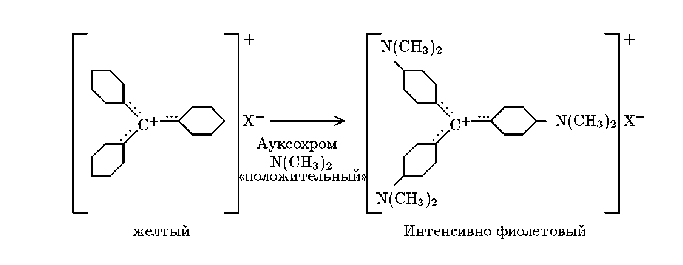
\includegraphics[scale=0.7]{Ris/ris_eps/ris3_05b.eps}}}

\vskip -2mm \leftskip 0cm Если окраска определяется анионом, то
роль << отрицательных ауксохромов>> играют другие группы: $\rm
NO$, $\rm NO_2$, $\rm SO_2$, $\rm -N=N-$ и др. Например:

\vskip 3mm
\centerline{\hbox{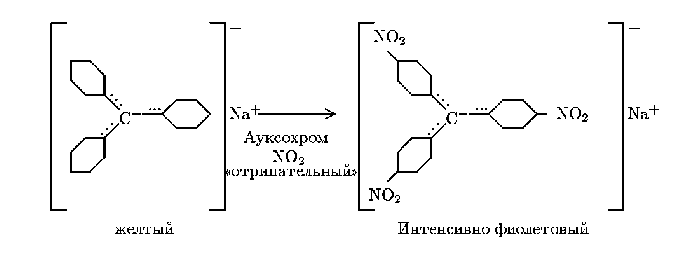
\includegraphics[scale=0.7]{Ris/ris_eps/ris3_05c.eps}}}

\vskip -2mm \leftskip 0cm {\ris Таблица 3.1. Органические
хромофоры.}

\vskip 3mm
\centerline{\hbox{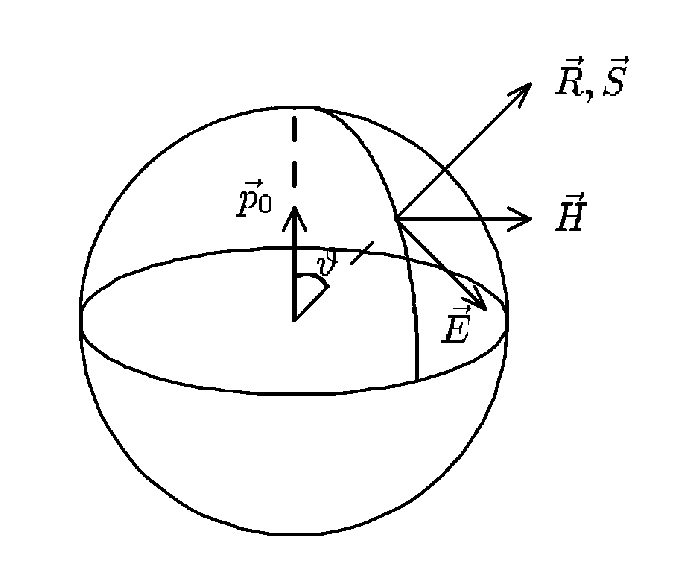
\includegraphics[scale=0.7]{Ris/ris_eps/ris3_01.eps}}}

\leftskip 0cm Связь между цветностью, т.е. положением полосы
поглощения, и химическим строением сложных молекул --- одна из
важных проблем теоретической химии. Следуя монографии А. Н.
Теренина (см. рис 3.6), показывающей соотношение между положением
полосы поглощения в видимом спектре и цветом пропускания ---
окраской вещества, рассмотрим особенности строения красителей
более подробно.

\vskip 3mm
\centerline{\hbox{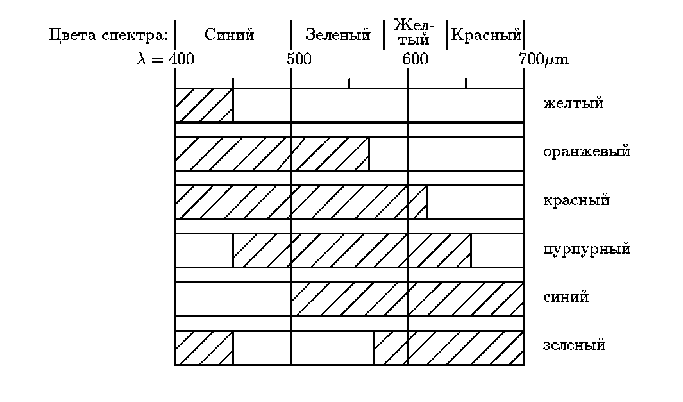
\includegraphics[scale=0.7]{Ris/ris_eps/ris3_06.eps}}}

\leftskip 0cm \centerline{\ris Рис. 3.6. Положение полос
поглощения и окраска (по А. Н. Теренину).} \vskip 2mm

Большинство сильно окрашенных органических соединений содержит
ненасыщенные циклические группировки с обобществленными
$\pi$-электронами, например:

\vskip 3mm
\centerline{\hbox{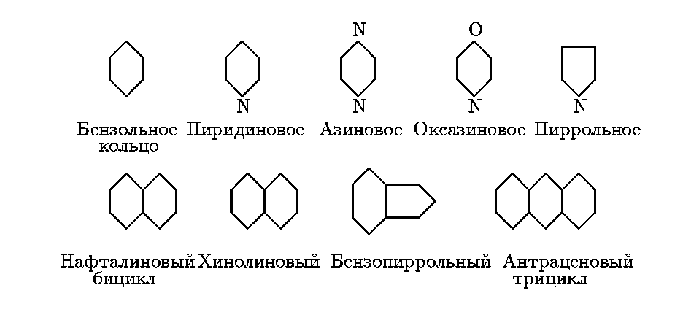
\includegraphics[scale=0.7]{Ris/ris_eps/ris3_06a.eps}}}

\leftskip 0cm В молекуле эти циклы связаны друг с другом или через
посредство некоторого центрального атома (например,
трифенилметановые красители), или цепочками сопряженных связей,
как например:
\begin{plain}
$$\eqalign{
&{\rm -N=N-}\hskip 7mm{\rm -CH=CH-CH=CH-}\hskip 7mm{\rm
-CH=N-CH=N-}\cr &{\rm азогруппа}\hskip 10mm{\rm полиметиновая\
цепь}\hskip 14mm{\rm азометиновая\ цепь} }$$
\end{plain}
Таким образом,
красители представляют собой сложные системы сопряженных
$\pi$-связей, взаимодействующих с циклическими системами
$\pi$-связей ароматического типа. Сопряжение определяет плоское
строение молекул красителей. Большинство красителей представлено
положительными и отрицательными ионами. Необходимо подчеркнуть,
что многие красители обладают свойствами индикаторов
--- меняют свой цвет при изменении концентрации водородных ионов
в окружающей среде. Например, в кислой среде метилоранж имеет
красный цвет, а в щелочной --- желтый. Фенолфталеин, относящийся к
группе ксантеновых красителей, имеет в щелочной среде ярко
пурпурный цвет, а в кислой среде --- бесцветен. Иными словами,
положение полосы поглощения существенным образом зависит от заряда
иона красителя. Способность молекулы красителя образовывать
положительные и отрицательные ионы определяется ионогенными
свойствами ауксохромных групп. Такие группы, как $\rm NH$ или $\rm
HR_2$, характеризуются основными свойствами, группы $\rm OH$ (в
феноле) и $HSO_3$ --- кислыми.

Непосредственная зависимость цветности от сопряжения $\pi$-связей
в красителях может быть иллюстрирована тем фактом, что при
гидрировании некоторых красителей, при уничтожении $\pi$-связей
получаются бесцветные соединения.

Таким образом, строение молекулы красителя обычно характеризуется
двумя важнейшими факторами: сопряжением $\pi$-связей и ионизацией.
Первый фактор практически обязателен для того, чтобы органическое
соединение обладало интенсивной полосой поглощения в видимой
области. Второй фактор может и не иметь места, хотя всегда
способствует появлению окраски.
